%% Preamble 
\documentclass[11pt,a4paper]{article}
\usepackage[utf8]{inputenc}
\usepackage[T1]{fontenc}
\usepackage{lmodern}
\usepackage[margin=25mm]{geometry}
\usepackage{amsmath,amssymb,mathtools,bm,array,xcolor,booktabs,longtable}
\usepackage{tikz,microtype,enumitem}
\usepackage[nolist]{acronym}
\usetikzlibrary{arrows.meta,positioning,fit}
\usepackage[colorlinks=true,linkcolor=blue!50!black,urlcolor=blue!50!black]{hyperref}
\newenvironment{example}[1]{\par\medskip\noindent\textbf{Worked example: #1.}\ }{\par\medskip}
\setlist[itemize]{noitemsep}
\numberwithin{equation}{section}
\setcounter{tocdepth}{1}

%%%%%%%%%%%%%%%%%%%%%%%%%%%%%%%%%%%%%%%%%%%%%%%%%%%%%%%%%%%%
% MIMO Communications - Common LaTeX Commands
%%%%%%%%%%%%%%%%%%%%%%%%%%%%%%%%%%%%%%%%%%%%%%%%%%%%%%%%%%%%
% Required packages:
% \usepackage{amsmath,amssymb,amsfonts}
% \usepackage{mathtools}
% \usepackage{bm}
% \usepackage{array}
% \usepackage{xcolor}
%
% Convention:
% - Scalars: italic
% - Vectors/matrices: bold lowercase/uppercase
% - Sets: calligraphic
% - Descriptive indices: \mathsf
% - Matrix transpose markers: \mathsf
% - Named mathematical operators: upright
%%%%%%%%%%%%%%%%%%%%%%%%%%%%%%%%%%%%%%%%%%%%%%%%%%%%%%%%%%%%


%%%%%%%%%%%%%%%%%%%%%%%%%%%%%%%%%%%%%%%%%%%%%%%%%%%%%%%%%%%%
% 1. REVIEW AND EDITING
%%%%%%%%%%%%%%%%%%%%%%%%%%%%%%%%%%%%%%%%%%%%%%%%%%%%%%%%%%%%

% Display old text [blue] and proposed text [red]
\newcommand{\Review}[2]{%
	{\color{blue}[#1]}{\color{red}[#2]}}

% Display corrected versions
\newcommand{\Fixed}[2]{%
	{\color{orange}[#1]}{\color{green}[#2]}}

% Show only the accepted version (first argument)
\newcommand{\Done}[2]{#1}

% Comments and notes
\newcommand{\Response}[1]{{\color{magenta}[#1]}}
\newcommand{\Note}[1]{{\color{blue}[#1]}}


%%%%%%%%%%%%%%%%%%%%%%%%%%%%%%%%%%%%%%%%%%%%%%%%%%%%%%%%%%%%
% 2. GENERAL UTILITIES
%%%%%%%%%%%%%%%%%%%%%%%%%%%%%%%%%%%%%%%%%%%%%%%%%%%%%%%%%%%%

% Fixed-width table columns with proper line breaks
\newcolumntype{C}[1]{>{\centering\arraybackslash}p{#1}}
\newcolumntype{R}[1]{>{\raggedleft\arraybackslash}p{#1}}
\newcolumntype{L}[1]{>{\raggedright\arraybackslash}p{#1}}

% Display literal LaTeX text
\newcommand{\ttplain}[1]{\texttt{\detokenize{#1}}}

% Underbraces for expressions in matrices/arrays
\newcommand{\undermat}[2]{%
	\makebox[0pt][l]{$%
		\smash{%
			\underbrace{%
				\phantom{\begin{matrix}#2\end{matrix}}%
			}_{\text{$#1$}}%
		}$}#2}

\newcommand{\coolunder}[2]{%
	\mathrlap{%
		\smash{%
			\underbrace{%
				\phantom{\begin{matrix}#2\end{matrix}}%
			}_{\mbox{$#1$}}%
		}%
	}#2}


%%%%%%%%%%%%%%%%%%%%%%%%%%%%%%%%%%%%%%%%%%%%%%%%%%%%%%%%%%%%
% 3. CROSS-REFERENCING
%%%%%%%%%%%%%%%%%%%%%%%%%%%%%%%%%%%%%%%%%%%%%%%%%%%%%%%%%%%%

\newcommand{\figref}[1]{Figure.~\ref{#1}}
\newcommand{\secref}[1]{Section~\ref{#1}}
\newcommand{\chapref}[1]{Chapter~\ref{#1}}
\newcommand{\theref}[1]{Theorem~\ref{#1}}
\newcommand{\appref}[1]{Appendix~\ref{#1}}
\newcommand{\tabref}[1]{Table~\ref{#1}}

% Define if not already provided by another package
\providecommand{\algref}[1]{}
\renewcommand{\algref}[1]{Algorithm~\ref{#1}}
% Additional packages for notation tables
\usepackage{longtable}
\usepackage{array}
%% MATH NOTATION
%%%%%%%%%%%%%%%%%%%%%%%%%%%%%%%%%%%%%%%%%%%%%%%%%%%%%%%%%%%%
% 4. MATHEMATICAL OPERATORS AND DELIMITERS
%%%%%%%%%%%%%%%%%%%%%%%%%%%%%%%%%%%%%%%%%%%%%%%%%%%%%%%%%%%%

% Ceiling and floor (mathtools)
\DeclarePairedDelimiter{\ceil}{\lceil}{\rceil}
\DeclarePairedDelimiter{\floor}{\lfloor}{\rfloor}

% Optimization operators
\DeclareMathOperator*{\argmax}{arg\,max}
\DeclareMathOperator*{\argmin}{arg\,min}
\DeclareMathOperator*{\argfirst}{arg\,first}

% Angle/phase of complex quantity
% Overrides any existing \ang definition
\providecommand{\ang}[1]{}
\renewcommand{\ang}[1]{%
	\operatorname{angle}\left(#1\right)}

% Definition symbol
\newcommand{\define}{\triangleq}

% Delimiters (legacy commands)
\newcommand{\LeftP}{\left\lbrace}
\newcommand{\RightP}{\right\rbrace}
\newcommand{\LeftPD}{\left(}
\newcommand{\RightPD}{\right)}

% Additional delimiters
\newcommand{\Abs}[1]{\left|#1\right|}
\newcommand{\inner}[2]{%
	\left\langle #1,#2\right\rangle}


%%%%%%%%%%%%%%%%%%%%%%%%%%%%%%%%%%%%%%%%%%%%%%%%%%%%%%%%%%%%
% 5. SETS AND NUMBER FIELDS
%%%%%%%%%%%%%%%%%%%%%%%%%%%%%%%%%%%%%%%%%%%%%%%%%%%%%%%%%%%%

\newcommand{\compl}{\mathbb{C}}   % Complex field
\newcommand{\real}{\mathbb{R}}    % Real field
\newcommand{\intg}{\mathbb{Z}}    % Integers
\newcommand{\galois}{\mathbb{F}_2} % Binary finite field

% Calligraphic sets
\newcommand{\set}[1]{\mathcal{#1}}


%%%%%%%%%%%%%%%%%%%%%%%%%%%%%%%%%%%%%%%%%%%%%%%%%%%%%%%%%%%%
% 6. VECTORS AND MATRICES
%%%%%%%%%%%%%%%%%%%%%%%%%%%%%%%%%%%%%%%%%%%%%%%%%%%%%%%%%%%%

% Bold lowercase vectors and uppercase matrices
\newcommand{\ma}[1]{\bm{#1}}

% Element indexing
\newcommand{\IndexM}[3]{#1\left[#2,#3\right]}
\newcommand{\IndexV}[2]{#1\left[#2\right]}

% Norms
\newcommand{\Norm}[1]{\left\|#1\right\|}
\newcommand{\NormTwo}[1]{\left\|#1\right\|_2}
\newcommand{\frob}[1]{\left\|#1\right\|_{\mathsf{F}}}

% Matrix operations
\newcommand{\inv}[1]{{#1}^{-1}}
\newcommand{\pinv}[1]{{#1}^{+}}        % Pseudoinverse
\newcommand{\mT}[1]{{#1}^{\mathsf{T}}} % Transpose
\newcommand{\mH}[1]{{#1}^{\mathsf{H}}} % Hermitian transpose
\newcommand{\mC}[1]{{#1}^{*}}         % Complex conjugate

% Matrix properties and functions
\newcommand{\trace}[1]{%
	\operatorname{tr}\left(#1\right)}
\newcommand{\rank}[1]{%
	\operatorname{rank}\left(#1\right)}
\newcommand{\Cond}[1]{%
	\operatorname{cond}\left(#1\right)}
\newcommand{\Det}[1]{%
	\operatorname{det}\left(#1\right)}
\newcommand{\diag}[1]{%
	\operatorname{diag}\left(#1\right)}

% Alias for compatibility
\newcommand{\diagM}[1]{\diag{#1}}

% Vector subspaces
\newcommand{\Span}[1]{%
	\operatorname{span}\left(#1\right)}
\newcommand{\Null}[1]{%
	\operatorname{null}\left(#1\right)}
\newcommand{\Range}[1]{%
	\operatorname{range}\left(#1\right)}

% Vectorization and reshaping
\newcommand{\Vect}[1]{%
	\operatorname{vec}\left(#1\right)}
\newcommand{\unvec}[3]{%
	\operatorname{unvec}_{#2\times #3}\left(#1\right)}

% Matrix products
\newcommand{\elemProd}[2]{#1\odot #2}
\newcommand{\elemDiv}[2]{#1\oslash #2}
\newcommand{\kronProd}[2]{#1\otimes #2}


%%%%%%%%%%%%%%%%%%%%%%%%%%%%%%%%%%%%%%%%%%%%%%%%%%%%%%%%%%%%
% 7. PROBABILITY AND STATISTICS
%%%%%%%%%%%%%%%%%%%%%%%%%%%%%%%%%%%%%%%%%%%%%%%%%%%%%%%%%%%%

% Expectation and variance
\newcommand{\Ex}[1]{%
	\mathbb{E}\left[#1\right]}
\newcommand{\Var}[1]{%
	\operatorname{Var}\left[#1\right]}

% Covariance and correlation
\newcommand{\Cov}[2]{%
	\operatorname{Cov}\left(#1,#2\right)}
\newcommand{\Corr}[2]{%
	\operatorname{Corr}\left(#1,#2\right)}

% Probability of an event
\newcommand{\Prob}[1]{%
	\Pr\left(#1\right)}

% Mean-square error
\newcommand{\MSE}[1]{%
	\operatorname{MSE}\left(#1\right)}

% Distribution notation
\newcommand{\Normal}{\mathcal{N}}
\newcommand{\CNormal}{\mathcal{CN}}

% Complex signal operations
\newcommand{\RE}[1]{%
	\operatorname{Re}\left\{#1\right\}}
\newcommand{\IM}[1]{%
	\operatorname{Im}\left\{#1\right\}}


%%%%%%%%%%%%%%%%%%%%%%%%%%%%%%%%%%%%%%%%%%%%%%%%%%%%%%%%%%%%
% 8. SIGNAL PROCESSING OPERATIONS
%%%%%%%%%%%%%%%%%%%%%%%%%%%%%%%%%%%%%%%%%%%%%%%%%%%%%%%%%%%%

% Fourier transform
\newcommand{\FT}[1]{%
	\mathcal{F}\left\{#1\right\}}

% Circular convolution
\newcommand{\circConv}[2]{#1\circledast #2}

% Modulo reduction notation
\newcommand{\modulo}[2]{%
	\left\langle #1\right\rangle_{#2}}

% Sinc function
\newcommand{\Sinc}[1]{%
	\operatorname{sinc}\left(#1\right)}


%%%%%%%%%%%%%%%%%%%%%%%%%%%%%%%%%%%%%%%%%%%%%%%%%%%%%%%%%%%%
% 9. MIMO DIMENSIONS AND INDICES
%%%%%%%%%%%%%%%%%%%%%%%%%%%%%%%%%%%%%%%%%%%%%%%%%%%%%%%%%%%%

% Subscripts t/r: transmit/receive interfaces
% Superscripts rf/a: RF-chain/antenna-element interfaces
% No superscript: effective digital signal ports
% S: number of data streams
%
% Descriptive indices are upright (\mathsf).
% Running mathematical indices are italic..

% Digital signal ports
\newcommand{\NT}{N_{\mathsf{t}}}
\newcommand{\NR}{N_{\mathsf{r}}}
\newcommand{\nT}{n_{\mathsf{t}}}
\newcommand{\nR}{n_{\mathsf{r}}}

% Data streams
\newcommand{\NS}{S}
\newcommand{\nS}{s}

% RF chains
\newcommand{\NTrf}{N_{\mathsf{t}}^{\mathsf{rf}}}
\newcommand{\NRrf}{N_{\mathsf{r}}^{\mathsf{rf}}}
\newcommand{\nTrf}{n_{\mathsf{t}}^{\mathsf{rf}}}
\newcommand{\nRrf}{n_{\mathsf{r}}^{\mathsf{rf}}}

% Physical antenna elements
\newcommand{\NTa}{N_{\mathsf{t}}^{\mathsf{a}}}
\newcommand{\NRa}{N_{\mathsf{r}}^{\mathsf{a}}}
\newcommand{\nTa}{n_{\mathsf{t}}^{\mathsf{a}}}
\newcommand{\nRa}{n_{\mathsf{r}}^{\mathsf{a}}}


%%%%%%%%%%%%%%%%%%%%%%%%%%%%%%%%%%%%%%%%%%%%%%%%%%%%%%%%%%%%
% 10. MIMO PRECODING AND COMBINING MATRICES
%%%%%%%%%%%%%%%%%%%%%%%%%%%%%%%%%%%%%%%%%%%%%%%%%%%%%%%%%%%%

% Digital precoding and combining
\newcommand{\FD}{\ma{F}_{\mathsf{D}}}
\newcommand{\WD}{\ma{W}_{\mathsf{D}}}

% Analog precoding and combining
\newcommand{\FA}{\ma{F}_{\mathsf{A}}}
\newcommand{\WA}{\ma{W}_{\mathsf{A}}}


% MIMO channel representations

\newcommand{\Ha}{\ma{H}_{\mathsf{a}}}
% Antenna-level channel (physical antenna elements)

\newcommand{\Hrf}{\ma{H}_{\mathsf{rf}}}
% Effective channel after analog TX/RX processing


% H_a: Physical antenna-to-antenna channel
% H_rf: Effective channel between RF-chain interfaces
% H: Effective channel between digital signal ports
% H_s: Effective channel between data streams
%
% H_rf = W_A^H H_a F_A
% H    = W_D^H H_rf F_D
% H_s  = W^H H F


\newcommand{\Hs}{\ma{H}_{\mathsf{s}}}
% Effective stream-level channel after digital
% precoding and combining

% Diversity and multiplexing performance
\providecommand{\odiv}{o_{\mathsf{div}}}   % Diversity order
\providecommand{\gmux}{g_{\mathsf{mux}}}   % Multiplexing gain


%%%%%%%%%%%%%%%%%%%%%%%%%%%%%%%%%%%%%%%%%%%%%%%%%%%%%%%%%%%%
% 11. SIGNAL ENERGY AND NOISE
%%%%%%%%%%%%%%%%%%%%%%%%%%%%%%%%%%%%%%%%%%%%%%%%%%%%%%%%%%%%

\newcommand{\Es}{E_{\mathsf{s}}} % Energy per symbol
\newcommand{\Ed}{E_{\mathsf{d}}} % Total energy

\newcommand{\Eb}{E_{\mathsf{b}}} % Energy per bit

% Noise power spectral density parameter
\newcommand{\Nzero}{N_{0}}

\newcommand{\Ptx}{P_{\mathsf{t}}}
\newcommand{\Prx}{P_{\mathsf{r}}}


%%%%%%%%%%%%%%%%%%%%%%%%%%%%%%%%%%%%%%%%%%%%%%%%%%%%%%%%%%%%
% 12. COMMUNICATION METRICS AND ALGORITHMS
%%%%%%%%%%%%%%%%%%%%%%%%%%%%%%%%%%%%%%%%%%%%%%%%%%%%%%%%%%%%

\newcommand{\SNR}{\mathsf{SNR}}
\newcommand{\SINR}{\mathsf{SINR}}
\newcommand{\CSI}{\mathsf{CSI}}

% Combining and precoding
\newcommand{\MRT}{\mathsf{MRT}}
\newcommand{\MRC}{\mathsf{MRC}}
\newcommand{\ZF}{\mathsf{ZF}}
\newcommand{\LMMSE}{\mathsf{LMMSE}}

% Additional commonly used methods
\newcommand{\LS}{\mathsf{LS}}
\newcommand{\MMSE}{\mathsf{MMSE}}
\newcommand{\ML}{\mathsf{ML}}
\newcommand{\MAP}{\mathsf{MAP}}
\newcommand{\RZF}{\mathsf{RZF}}





%%%%%%%%%%%%%%%%%%%%%%%%%%%%%%%%%%%%%%%%%%%%%%%%%%%%%%%%%%%%
% End of common notation
%%%%%%%%%%%%%%%%%%%%%%%%%%%%%%%%%%%%%%%%%%%%%%%%%%%%%%%%%%%%

% Channel-rank abbreviation consistent with Lecture 01: $\RH=R_{\ma{H}}$.
\providecommand{\RH}{R_{\ma{H}}}
\title{MIMO Communications\\Lecture 03: Point-to-Point MIMO Channel Statistics and Performance}
\author{Ahmad Nimr}
\date{Winter Semester 2026/27}

\begin{document}
% Register shared acronyms after the document begins.
\begin{acronym}
	\acro{p2p}[P2P]{point-to-point}
	\acro{mimo}[MIMO]{multiple-input multiple-output}
	\acro{siso}[SISO]{single-input single-output}
	\acro{simo}[SIMO]{single-input multiple-output}
	\acro{miso}[MISO]{multiple-input single-output}
	\acro{mrc}[MRC]{maximum ratio combining}
	\acro{mrt}[MRT]{maximum ratio transmission}
	\acro{zf}[ZF]{zero forcing}
	\acro{lmmse}[LMMSE]{linear minimum mean-square error}
	\acro{mmse}[MMSE]{minimum mean-square error}
	\acro{svd}[SVD]{singular value decomposition}
	\acro{evd}[EVD]{eigenvalue decomposition}
	\acro{snr}[SNR]{signal-to-noise ratio}
	\acro{sinr}[SINR]{signal-to-interference-plus-noise ratio}
	\acro{csi}[CSI]{channel state information}
	\acro{csir}[CSIR]{channel state information at the receiver}
	\acro{csit}[CSIT]{channel state information at the transmitter}
	\acro{rf}[RF]{radio frequency}
	\acro{qpsk}[QPSK]{quadrature phase-shift keying}
	\acro{awgn}[AWGN]{additive white Gaussian noise}
	\acro{psd}[PSD]{power spectral density}
	\acro{map}[MAP]{maximum a posteriori}
	\acro{mse}[MSE]{mean squared error}
	\acro{ls}[LS]{least squares}
	\acro{ml}[ML]{maximum likelihood }
	\acro{bpsk}[BPSK]{binary phase-shift keying}
	\acro{iid}[IID]{independent and identically distributed}
	\acro{los}[LOS]{line of sight}
	\acro{ostbc}[OSTBC]{orthogonal space-time block code}
	\acro{stbc}[STBC]{space-time block code}
	\acro{dmt}[DMT]{diversity--multiplexing tradeoff}
	\acro{pdf}[PDF]{probability density function}
	\acro{mumimo}[MU-MIMO]{multiuser multiple-input multiple-output}
	\acro{ul}[UL]{uplink}
	\acro{dl}[DL]{downlink}
	\acro{fdma}[FDMA]{frequency-division multiple access}
	\acro{tdma}[TDMA]{time-division multiple access}
	\acro{sdma}[SDMA]{space-division multiple access}
	\acro{bs}[BS]{base station}
	\acro{mac}[MAC]{multiple-access channel}
	\acro{bc}[BC]{broadcast channel}
	\acro{rzf}[RZF]{regularized zero forcing}
	\acro{sic}[SIC]{successive interference cancellation}
	\acro{dpc}[DPC]{dirty-paper coding}
	\acro{dof}[DoF]{degrees of freedom}
	\acro{tdd}[TDD]{time-division duplex}
	\acro{fdd}[FDD]{frequency-division duplex}
	\acro{ap}[AP]{access point}
	\acro{cpu}[CPU]{central processing unit}
	\acro{comp}[CoMP]{coordinated multipoint}
	\acro{cscg}[CSCG]{circularly symmetric complex Gaussian}
	\acro{mu}[MU]{multi-user}
	\acro{se}[SE]{spectral efficiency}
\end{acronym}

\acresetall
\maketitle
\begin{abstract}
Lecture~02 characterized a fixed point-to-point channel. This lecture asks how often useful spatial channels occur and how reliably they support a desired rate. It introduces Rayleigh, Rician, and spatially correlated channel models, connects their statistics to singular values and useful spatial dimensions, and distinguishes instantaneous rate, ergodic rate, outage, and error probability. Receive and transmit diversity are analyzed under explicit channel-knowledge assumptions. Analytic examples and numerical comparisons show why channel gain, rank, correlation, and reliability must be examined together.
\end{abstract}
\acresetall
\tableofcontents
\newpage

\section{From deterministic channels to random channels}
\label{sec:random}

\subsection{Learning objectives and connection to Lecture 02}

This lecture introduces statistical MIMO channel models
and their impact on spatial properties, achievable rate,
and reliability. Emphasis is placed on channel normalization,
channel state information, ergodic rate, outage, and diversity.

The effective digital-port model and normalization of
Lecture~02 are retained:
\begin{align}
	\ma{y}&=\ma{H}\ma{x}+\ma{v},&
	\ma{x}&=\ma{F}\ma{d},&
	\ma{y}_{\mathsf c}&=\mH{\ma{W}}\ma{y},
	\label{eq:model}\\
	\ma{v}&\sim\CNormal(\ma{0},\sigma_v^2\ma{I}_{\NR}),&
	\ma{R}_d&=\Ed\ma{I}_{\NS},&
	\rho&=\Ed/\sigma_v^2.
	\nonumber
\end{align}
Here $\ma{H}\in\compl^{\NR\times\NT}$,
$\ma{F}\in\compl^{\NT\times\NS}$, and
$\ma{W}\in\compl^{\NR\times\NS}$.
The stream precoder satisfies $\frob{\ma{F}}^2\leq1$,
such that
\begin{equation*}
	\ma{R}_x=\Ed\ma{F}\mH{\ma{F}},
	\qquad
	\trace{\ma{R}_x}\leq\Ed.
\end{equation*}
The matrices $\ma{F}$ and $\ma{W}$ represent stream
precoding and combining, whereas $\ma{H}$ includes
the preceding frontend transformations.
The noise is assumed independent of the data and
channel, and spatially white unless otherwise stated.
The budget $\Ed$ specifies energy per complex channel use.

\subsection{Realizations and distributions}

A channel realization $\ma{H}=\ma{H}_0$ is a fixed
matrix to which the results of Lecture~02 apply.
A statistical channel model describes the distribution
of possible realizations. Even realizations from the same
distribution may have substantially different singular
values and conditioning.

\begin{example}{Spatial variation of a wireless channel}
	Consider a receiver moving through different locations
	within a given area, while the transmitter remains fixed.
	At each position $\ma{p}$, a channel realization
	$\ma{H}(\ma{p})$ is observed due to variations in
	propagation distances and multipath interference.
	%
	Channel statistics can be characterized by measuring
	$\ma{H}(\ma{p})$ at representative locations and
	studying the distribution of the resulting matrices.
	%
	These statistics also describe the performance experienced
	by a receiver moving through the area. For example,
	the average achievable rate characterizes the mean
	performance, while the outage probability indicates
	how frequently a target rate cannot be supported.
	%
	This interpretation assumes representative spatial sampling
	and approximately stationary channel statistics within
	the considered area.
\end{example}

\paragraph{From channel realizations to performance distributions.}
For a specified transmission scheme, the achievable rate
$R(\ma{H})$ becomes a random variable.
Its statistical performance can be characterized by
the average rate $\Ex{R(\ma{H})}$ and the probability
that a target rate $R_0$ cannot be supported.
These measures depend on the transmission strategy
and the channel variations experienced by a codeword.

A block-fading channel is modeled as
\begin{equation}
	\ma{y}_b[n]
	=\ma{H}_b\ma{x}_b[n]+\ma{v}_b[n],
	\qquad n=1,\ldots,T_{\mathsf c},
\end{equation}
where the channel remains constant within each block
and may change between blocks.
The blocks may be statistically independent or correlated,
depending on the propagation and mobility.
Whether a codeword spans one or several blocks determines
the appropriate ergodic or outage interpretation.

\subsection{Large-scale and small-scale fading}

The channel is decomposed into a large-scale power gain
and normalized small-scale fading:
\begin{equation}\label{eq:beta}
	\boxed{
		\ma{H}=\sqrt{\beta}\,\breve{\ma{H}},
		\qquad \beta>0.
	}
\end{equation}
The coefficient $\beta$ accounts for path loss and,
when included, shadowing.
The matrix $\breve{\ma{H}}$ describes the typically
faster amplitude and phase variations due to multipath
propagation.

Unless stated otherwise, $\beta$ is fixed and
the small-scale channel is normalized as
\begin{equation}\label{eq:normalization}
	\boxed{
		\Ex{\frob{\breve{\ma{H}}}^2}=\NT\NR,
		\qquad
		\Ex{\frob{\ma{H}}^2}=\beta\NT\NR.
	}
\end{equation}
Thus, the average squared channel gain per matrix
entry is $\beta$, when averaged over all entries.
Individual entries need not have identical statistics.

This normalization includes the gain from additional
receive ports in antenna-count comparisons.
Comparisons at equal total channel energy represent
a different normalization.
Individual channel realizations must not be normalized
to a fixed Frobenius norm when fading reliability
is evaluated, since this would alter the fading statistics.

\begin{example}{Effect of large-scale attenuation}
	Consider the scalar Rayleigh channel
	$h=\sqrt{\beta}\,\breve{h}$, where
	$\breve{h}\sim\CNormal(0,1)$.
	The instantaneous received \ac{snr} is
	\begin{equation*}
		\rho_{\mathsf r}
		=\rho\beta\Abs{\breve{h}}^2.
	\end{equation*}
	Reducing $\beta$ from $1$ to $0.1$ decreases
	the average received \ac{snr} by $10$~dB,
	without changing the normalized fading distribution
	or its diversity order.
\end{example}

\subsection{Instantaneous and statistical channel knowledge}

Instantaneous \ac{csi} describes the current channel
realization, whereas statistical \ac{csi} describes
parameters such as mean gains and spatial covariances.
Perfect \ac{csir} is assumed for coherent reception.
Three transmitter-information cases are considered:
no instantaneous \ac{csit}, statistical \ac{csit},
and perfect instantaneous \ac{csit}.

For a fixed precoder, the transmit covariance is
\begin{equation*}
	\ma{R}_x=\Ed\ma{F}\mH{\ma{F}}.
\end{equation*}
With instantaneous channel adaptation, it becomes
\begin{equation*}
	\ma{R}_x(\ma{H})
	=\Ed\ma{F}(\ma{H})\mH{\ma{F}(\ma{H})}.
\end{equation*}
The same short-term energy constraint is imposed
for every realization:
\begin{equation}\label{eq:shortpower}
	\boxed{
		\trace{\ma{R}_x(\ma{H})}\leq\Ed.
	}
\end{equation}
Under this constraint, water-filling allocates energy
across spatial modes within each channel realization,
without transferring energy between fading blocks.

A long-term constraint,
$\Ex{\trace{\ma{R}_x(\ma{H})}}\leq\Ed$,
also permits energy adaptation across blocks and
leads to a different optimization problem.

\paragraph{Spatial correlation.}
Channel coefficients may be statistically correlated
due to shared scattering, similar propagation directions,
or antenna responses.
Spatial correlation describes dependencies across
channel realizations and is distinct from the
conditioning of one particular matrix.
Statistical correlation models are introduced next;
geometry-based models are addressed later in the course.



\section{Statistical MIMO channel models}
\label{sec:models}

\subsection{Independent Rayleigh fading}

Consider a random matrix
$\ma{H}_{\mathsf w}\in\compl^{\NR\times\NT}$
with \ac{iid} entries
\begin{equation}\label{eq:rayleigh}
	[\ma{H}_{\mathsf w}]_{\nR\nT}
	=\frac{a_{\nR\nT}+jb_{\nR\nT}}{\sqrt{2}}
	\sim\CNormal(0,1),
\end{equation}
where $a_{\nR\nT},b_{\nR\nT}\sim\Normal(0,1)$ are
mutually independent real Gaussian variables.

The independent Rayleigh channel is modeled as
\begin{equation*}
	\boxed{
		\ma{H}=\sqrt{\beta}\,\ma{H}_{\mathsf w}.
	}
\end{equation*}
Each normalized coefficient has zero mean and unit
variance. Its magnitude
$r=\Abs{[\ma{H}_{\mathsf w}]_{ij}}$
follows the Rayleigh distribution,
\begin{equation*}
	f_r(r)=2r e^{-r^2},\qquad r\geq0,
\end{equation*}
while its squared magnitude is exponentially
distributed:
\begin{equation}\label{eq:exponential}
	f_{r^2}(u)=e^{-u},\quad u\geq0,
	\qquad
	\Prob{r^2<x}=1-e^{-x},\quad x\geq0.
\end{equation}

The zero-mean Gaussian model approximates the
superposition of many unresolved propagation
contributions without a dominant coherent component.
Spatial independence is an idealization; temporal
independence must be specified separately.


\subsection{Rician fading and deterministic components}

A normalized deterministic component
$\ma{H}_{\mathsf{det}}$ can be combined with
random scattering:
\begin{equation}\label{eq:rician}
	\boxed{
		\ma{H}=\sqrt{\beta}\left(
		\sqrt{\frac{\kappa}{\kappa+1}}\,
		\ma{H}_{\mathsf{det}}
		+\sqrt{\frac{1}{\kappa+1}}\,
		\ma{H}_{\mathsf w}
		\right),\qquad \kappa\geq0.
	}
\end{equation}
The components satisfy
\begin{equation*}
	\frob{\ma{H}_{\mathsf{det}}}^2
	=\NT\NR,
	\qquad
	\Ex{\frob{\ma{H}_{\mathsf w}}^2}
	=\NT\NR.
\end{equation*}
Thus, $\kappa$ is the ratio of deterministic to average
scattered power, and the channel normalization is
preserved:
\begin{equation*}
	\Ex{\frob{\ma{H}}^2}
	=\beta\NT\NR.
\end{equation*}

The channel mean is
\begin{equation*}
	\Ex{\ma{H}}
	=\sqrt{\frac{\beta \kappa}{\kappa+1}}\,
	\ma{H}_{\mathsf{det}},
\end{equation*}
and the scattered component has covariance scaled
by $\beta/(\kappa+1)$.
The parameter $\kappa$ represents the total component
power ratio; individual links may have different
local Rician factors.

At $\kappa=0$, independent Rayleigh fading is recovered.
As $\kappa\to\infty$, the channel approaches
$\sqrt{\beta}\ma{H}_{\mathsf{det}}$.
A stronger deterministic component may reduce
power fluctuations, but its spatial structure
determines the available channel modes.

\paragraph{Physical interpretation.}
The deterministic matrix may describe a stable
direct path or other coherent propagation components.
Its structure depends on antenna geometry, responses,
and propagation conditions.

For example, a single separable propagation path
can be represented as
\begin{equation*}
	\ma{H}_{\mathsf{det}}
	=\alpha\ma{a}_{\mathsf r}
	\mH{\ma{a}_{\mathsf t}},
\end{equation*}
which has rank at most one.
More general propagation geometries can support
multiple modes. An arbitrary deterministic matrix
does not necessarily correspond to a single
physical propagation path.

\begin{example}{Same Rician factor, different spatial structure}
	\label{ex:rician}
	
	Consider two deterministic $2\times2$ matrices:
	\begin{equation*}
		\ma{H}_{\mathsf{det},1}
		=
		\begin{bmatrix}
			1&1\\1&1
		\end{bmatrix},
		\qquad
		\ma{H}_{\mathsf{det},2}
		=\sqrt{2}\ma{I}_2.
	\end{equation*}
	Both have squared Frobenius norm $4$, but their
	squared singular values differ:
	\begin{equation*}
		(4,0)
		\qquad\text{and}\qquad
		(2,2).
	\end{equation*}
	
	In the deterministic limit with $\beta=1$,
	isotropic transmission gives
	\begin{align*}
		R_1&=\log_2(1+2\rho),\\
		R_2&=2\log_2(1+\rho).
	\end{align*}
	With optimal instantaneous \ac{csit},
	the first channel achieves
	\begin{equation*}
		C_1=\log_2(1+4\rho),
	\end{equation*}
	while the second has the same capacity as its
	isotropic transmission rate.
	
	Thus, equal deterministic power and equal Rician
	factors do not imply equal spatial multiplexing
	capability. These examples represent mathematical
	channel structures, not necessarily single-path
	physical realizations.
\end{example}


\subsection{Correlated Rayleigh fading: the Kronecker model}

Spatial correlation can be introduced through
two Hermitian positive-semidefinite matrices:
\begin{equation*}
	\ma{R}_{\mathsf r}\in
	\compl^{\NR\times\NR},
	\qquad
	\ma{R}_{\mathsf t}\in
	\compl^{\NT\times\NT}.
\end{equation*}
Both are normalized to unit diagonal, giving
$\trace{\ma{R}_{\mathsf r}}=\NR$ and
$\trace{\ma{R}_{\mathsf t}}=\NT$.

The Kronecker channel model is
\begin{equation}\label{eq:kronecker}
	\boxed{
		\ma{H}=\sqrt{\beta}\,
		\ma{R}_{\mathsf r}^{1/2}
		\ma{H}_{\mathsf w}
		\ma{R}_{\mathsf t}^{1/2},
	}
\end{equation}
where the square roots are Hermitian
positive-semidefinite.
Identity correlation matrices recover independent
Rayleigh fading.

For column-wise vectorization, the channel covariance is
\begin{equation}\label{eq:vectorcov}
	\boxed{
		\Cov{\Vect{\ma{H}}}{\Vect{\ma{H}}}
		=\beta\,
		\kronProd{\mT{\ma{R}_{\mathsf t}}}
		{\ma{R}_{\mathsf r}}.
	}
\end{equation}
The transpose on the transmit factor follows
from the vectorization convention.

Equivalently, the elementwise covariance is
\begin{equation*}
	\Ex{h_{ij}h_{k\ell}^*}
	=\beta
	[\ma{R}_{\mathsf r}]_{ik}
	[\ma{R}_{\mathsf t}]_{\ell j}.
\end{equation*}

The average Gram matrices are
\begin{align}
	\Ex{\ma{H}\mH{\ma{H}}}
	&=\beta\NT\ma{R}_{\mathsf r},
	\\
	\Ex{\mH{\ma{H}}\ma{H}}
	&=\beta\NR\ma{R}_{\mathsf t}.
\end{align}
Consequently,
\begin{equation*}
	\Ex{\frob{\ma{H}}^2}
	=\beta
	\trace{\ma{R}_{\mathsf r}}
	\trace{\ma{R}_{\mathsf t}}
	=\beta\NT\NR.
\end{equation*}

The correlation factors describe normalized
spatial covariance structures rather than the
unnormalized average Gram matrices.


\paragraph{Generating correlated channel samples.}

For a Hermitian positive-semidefinite matrix,
the square root can be obtained by
eigendecomposition:
\begin{align*}
	\ma{R}
	&=\ma{Q}
	\diag{\lambda_1,\ldots,\lambda_n}
	\mH{\ma{Q}},\\
	\ma{R}^{1/2}
	&=\ma{Q}
	\diag{\sqrt{\lambda_1},\ldots,\sqrt{\lambda_n}}
	\mH{\ma{Q}}.
\end{align*}
This construction also applies to singular matrices.

Cholesky or other covariance factors may be used
instead. If
$\ma{R}_{\mathsf t}=\ma{L}_{\mathsf t}
\mH{\ma{L}_{\mathsf t}}$,
the transmit-side factor must appear as
$\mH{\ma{L}_{\mathsf t}}$ on the right.
Elementwise square roots do not provide a
valid matrix factorization in general.


\begin{example}{Correlation redistributes spatial power}
	\label{ex:corr}
	
	Consider
	\begin{equation}\label{eq:correlation}
		\ma{R}(\alpha)=
		\begin{bmatrix}
			1&\alpha\\
			\alpha&1
		\end{bmatrix},
		\qquad 0\leq\alpha\leq1.
	\end{equation}
	Its eigenvalues are
	\begin{equation*}
		\lambda_1=1+\alpha,\qquad
		\lambda_2=1-\alpha.
	\end{equation*}
	Their sum remains $2$, independently of $\alpha$.
	
	For $\alpha=0.9$, the eigenvalues are
	$(1.9,0.1)$, indicating strong concentration
	of statistical power in one direction.
	Both directions remain available, whereas
	$\alpha=1$ produces a rank-one covariance.
	
	For a complex correlation coefficient $c$,
	the off-diagonal entries are $c$ and $c^*$,
	with $\Abs{c}\leq1$, and the eigenvalues
	become $1\pm\Abs{c}$.
\end{example}


\subsection{Interpretation and limitations}

\paragraph{Correlation versus conditioning.}
Spatial covariance characterizes statistical
dependencies and average channel behavior.
In contrast, the singular values of $\ma{H}$
describe one particular realization.

Full-rank covariance factors can generate
poorly conditioned channel realizations.
Similarly, a well-conditioned realization
may have low overall channel gain.
Statistical performance therefore depends
on the distribution of channel realizations,
not only on their average covariance.

\paragraph{Limitations of the Kronecker model.}
The model separates transmit and receive
spatial correlations. General coupling
between departure and arrival directions
cannot always be represented by two
independent covariance factors.

The model also does not explicitly describe
antenna geometry, propagation delays,
Doppler, mutual coupling, or frequency dependence.
A deterministic mean may be combined with
correlated scattering, provided their powers
are normalized consistently.


\begin{example}{Full covariance versus Kronecker model}
	
	Consider a $3\times2$ channel with
	$\NR=3$, $\NT=2$, and $\beta=1$:
	\begin{equation*}
		\ma{H}=[\ma{h}_1,\ma{h}_2],
		\qquad
		\ma{h}_1,\ma{h}_2\in\compl^{3\times1}.
	\end{equation*}
	With column-wise vectorization, the full spatial
	covariance has dimension $6\times6$:
	\begin{equation*}
		\ma{C}_h
		=\Cov{\Vect{\ma{H}}}{\Vect{\ma{H}}}
		\in\compl^{6\times6}.
	\end{equation*}
	
	In the Kronecker model, this covariance is restricted to
	\begin{equation*}
		\ma{C}_h
		=\kronProd{\mT{\ma{R}_{\mathsf t}}}
		{\ma{R}_{\mathsf r}},
		\qquad
		\begin{cases}
			\ma{R}_{\mathsf t}\in\compl^{2\times2},\\
			\ma{R}_{\mathsf r}\in\compl^{3\times3}.
		\end{cases}
	\end{equation*}
	
	To illustrate the limitation, consider independent
	Gaussian channel columns with
	\begin{equation*}
		\ma{h}_1\sim\CNormal(\ma{0},\ma{R}_1),
		\qquad
		\ma{h}_2\sim\CNormal(\ma{0},\ma{R}_2),
	\end{equation*}
	where
	\begin{equation*}
		\ma{R}_1=
		\begin{bmatrix}
			1&0.5&0\\
			0.5&1&0\\
			0&0&1
		\end{bmatrix},
		\qquad
		\ma{R}_2=\ma{I}_3.
	\end{equation*}
	The full covariance is
	\begin{equation*}
		\boxed{
			\ma{C}_h=
			\begin{bmatrix}
				\ma{R}_1&\ma{0}\\
				\ma{0}&\ma{R}_2
			\end{bmatrix}.
		}
	\end{equation*}
	
	This is a valid spatial covariance with
	different receive-side correlation structures
	for the two transmit ports.
	
	However, with unit-diagonal correlation factors,
	the Kronecker model requires
	\begin{equation*}
		\ma{C}_h
		=
		\begin{bmatrix}
			\ma{R}_{\mathsf r}
			&[\ma{R}_{\mathsf t}]_{21}\ma{R}_{\mathsf r}\\
			[\ma{R}_{\mathsf t}]_{12}\ma{R}_{\mathsf r}
			&\ma{R}_{\mathsf r}
		\end{bmatrix}.
	\end{equation*}
	Both diagonal blocks must therefore be identical,
	which is impossible for $\ma{R}_1\neq\ma{R}_2$.
	
	Thus, the Kronecker model describes only a
	restricted class of spatial covariance structures,
	whereas the full covariance allows general
	dependencies between antenna links.
\end{example}
\paragraph{Uncorrelated does not imply independent.}
Second-order statistics do not uniquely determine
a non-Gaussian channel distribution.

For example, consider the keyhole model
\begin{equation*}
	\ma{H}=\ma{a}\mH{\ma{b}},
\end{equation*}
where $\ma{a}\in\compl^{\NR\times1}$ and
$\ma{b}\in\compl^{\NT\times1}$ are independent
random vectors with \ac{iid}
$\CNormal(0,1)$ entries.

The channel has rank one almost surely,
although
\begin{align*}
	\Ex{\ma{H}\mH{\ma{H}}}
	&=\NT\ma{I}_{\NR},\\
	\Ex{\mH{\ma{H}}\ma{H}}
	&=\NR\ma{I}_{\NT}.
\end{align*}
Its entries are uncorrelated but statistically
dependent and not jointly Gaussian.
Thus, uncorrelated channel coefficients
do not guarantee independent spatial modes.


\section{Channel properties and spatial degrees of freedom}
\label{sec:properties}

The rank and singular values introduced in Lecture~02
describe the spatial properties of a fixed channel.
For random channels, these properties may vary between
realizations and are characterized statistically.

\subsection{Rank and singular-value statistics}

For each channel realization, the compact \ac{svd} is
\begin{equation*}
	\ma{H}
	=\ma{U}_{H}\ma{\Sigma}_{H}\mH{\ma{V}_{H}},
	\qquad
	\ma{\Sigma}_{H}
	=\diag{\sigma_1,\ldots,\sigma_{\RH}},
\end{equation*}
where
$\sigma_1\geq\cdots\geq\sigma_{\RH}>0$.

For independent Rayleigh fading, the channel has
maximum rank almost surely:
\begin{equation}\label{eq:rank-rayleigh}
	\boxed{
		\Prob{\RH=\min(\NT,\NR)}=1.
	}
\end{equation}
However, maximum rank does not imply equally
strong spatial modes. In particular, the smallest
singular value may approach zero.
%
For the Kronecker model, let
\begin{equation*}
	q_{\mathsf r}=\rank{\ma{R}_{\mathsf r}},
	\qquad
	q_{\mathsf t}=\rank{\ma{R}_{\mathsf t}}.
\end{equation*}
The channel rank satisfies
\begin{equation}\label{eq:rank-kronecker}
	\boxed{
		\RH=\min(q_{\mathsf r},q_{\mathsf t})
		\quad\text{almost surely}.
	}
\end{equation}
Thus, full-rank correlation factors preserve
the maximum rank, whereas singular factors
restrict the available spatial dimensions.
%
For finite Rician factor $\kappa$, the channel
also has maximum rank almost surely when
the scattering component has full-dimensional
Gaussian statistics. In the deterministic limit
$\kappa\to\infty$, the rank is determined by
$\ma{H}_{\mathsf{det}}$.

\paragraph{Statistical interpretation.}
Although the exact rank is almost surely fixed
in these models, the singular values vary
between channel realizations.
%
Their distributions describe the occurrence of
strong and weak spatial modes. For example,
the distribution of the smallest singular value
indicates how frequently a channel becomes
nearly rank deficient, even when its exact
rank is maximal.


\subsection{Conditioning and effective rank}

For a channel with positive singular values,
the spectral condition number is
\begin{equation}\label{eq:condition}
	\mathsf{cond}_{H}
	=\frac{\sigma_1}{\sigma_{\RH}}.
\end{equation}
For a full-rank channel, a large
$\mathsf{cond}_{H}$ indicates strongly unequal
mode gains. A rank-deficient channel has
missing spatial dimensions, irrespective of
the conditioning within its nonzero subspace.
%
For linear \ac{zf} equalization, weak singular
directions cause noise enhancement.
Thus, the distribution of channel conditioning
affects the reliability of simultaneous
stream recovery.
%
Conditioning alone does not determine performance:
a channel such as $0.001\ma{I}_2$ is perfectly
conditioned but has very low gain.

\paragraph{Effective rank.}
The relative distribution of spatial power
can be described using the normalized
squared singular values
\begin{equation*}
	q_s
	=\frac{\sigma_s^2}
	{\sum_{\ell=1}^{\RH}\sigma_\ell^2},
	\qquad
	\sum_{s=1}^{\RH}q_s=1.
\end{equation*}
An entropy-based effective rank is defined as
\begin{equation}\label{eq:effectiverank}
	\boxed{
		r_{\mathsf{eff}}
		=\exp\left(
		-\sum_{s=1}^{\RH}q_s\ln q_s
		\right).
	}
\end{equation}
For a nonzero channel,
\begin{equation*}
	1\leq r_{\mathsf{eff}}\leq\RH.
\end{equation*}
It equals $\RH$ for equal positive mode gains
and approaches $1$ when one mode dominates.
%
Effective rank describes the balance of spatial
power, rather than the number of mathematically
independent modes. It is invariant to channel
scaling and does not account for noise or
transmit energy.
%
In contrast, the number of modes activated by
water-filling depends on the operating \ac{snr}.
Effective rank is therefore a descriptive
measure, not a direct capacity or stream-count
criterion.

\begin{example}{Rank, effective rank, and active modes}
	Consider a channel with squared singular values
	\begin{equation*}
		(\sigma_1^2,\sigma_2^2)=(1,0.01).
	\end{equation*}
	Its exact rank and condition number are
	\begin{equation*}
		\RH=2,\qquad \mathsf{cond}_{H}=10.
	\end{equation*}
	The effective rank is
	\begin{equation*}
		r_{\mathsf{eff}}\approx1.057.
	\end{equation*}
	With $\sigma_v^2=1$, water-filling allocates
	positive energy to the second mode only when
	\begin{equation*}
		\Ed>99.
	\end{equation*}
	Thus, two independent spatial modes exist,
	but the weaker mode is useful for optimal
	spatial multiplexing only at sufficiently
	high \ac{snr}.
\end{example}

\paragraph{Statistics of spatial properties.}
For a random channel, the condition number,
effective rank, and singular values are
random quantities.
%
Their distributions can be estimated from
channel realizations. For example,
$\Ex{r_{\mathsf{eff}}}$ describes the average
balance of spatial power, whereas
\begin{equation*}
	\Prob{\sigma_{\min}^2<\epsilon}
\end{equation*}
describes the probability that the smallest
singular-value gain falls below a threshold.
Here $\sigma_{\min} = \sigma_{\RH}$ is the smallest
singular value among the
$\min(\NT,\NR)$ singular values, including
zeros when the channel is rank deficient.
%
These statistics provide information about
the frequency of weak channel conditions,
but achievable rate and outage must still
be evaluated for a specified transmission
scheme.


\subsection{Antenna configuration and favorable channels}

Additional receive ports provide more observations,
while additional transmit ports provide more
possible transmit directions.
%
Under independent Rayleigh fading, increasing
the port counts can increase diversity and
the number of spatial modes.
With spatial correlation or restricted propagation,
these gains may be reduced.
%
The relation between antenna configuration and
channel statistics is described here through
statistical models. Its geometric interpretation
is developed later in the course.

\paragraph{What makes a channel favorable?}
The answer depends on the performance objective.
%
For a fixed total squared channel gain,
balanced singular-value gains favor
equal-energy spatial multiplexing.
Concentrating the gain into a dominant mode
can instead favor single-stream transmission
at low \ac{snr}.
%
For a random channel, reliable performance
additionally depends on how frequently weak
channel realizations occur.
Therefore, neither average channel gain,
effective rank, nor conditioning alone
fully characterizes statistical performance.



\section{Performance metrics}
\label{sec:metrics}

\subsection{Instantaneous achievable rate and transmission schemes}

For Gaussian signaling and perfect \ac{csir}, the achievable rate of a given channel realization is
\begin{equation}\label{eq:instant}
	R(\ma{H},\ma{R}_x)
	=\log_2\Det{\ma{I}_{\NR}
		+\sigma_v^{-2}\ma{H}\ma{R}_x\mH{\ma{H}}}.
\end{equation}
The rate depends on the channel realization and the selected transmission and reception scheme. The following cases are distinguished:

\begin{itemize}
	\item \textbf{Fixed isotropic transmission:} Equal energy is allocated to all transmit ports, without instantaneous \ac{csit}.
	\item \textbf{Statistical-CSIT transmission:} A fixed covariance is optimized using channel statistics, without adaptation to individual realizations.
	\item \textbf{Instantaneous-CSIT transmission:} Precoding and energy allocation are adapted to each realization, for example through \ac{svd} and water-filling.
	\item \textbf{Linear equalization:} A specified precoder is followed by receiver combining and separate stream decoding, which may achieve a lower rate than joint decoding.
\end{itemize}

\paragraph{Isotropic transmission.}
Without instantaneous \ac{csit}, an important benchmark is
\begin{equation}\label{eq:iso}
	\ma{R}_{x,\mathsf{iso}}
	=\frac{\Ed}{\NT}\ma{I}_{\NT},
	\qquad
	R_{\mathsf{iso}}(\ma{H})
	=\sum_{s=1}^{\RH}
	\log_2\left(1+\frac{\rho\sigma_s^2}{\NT}\right).
\end{equation}

\paragraph{Instantaneous-CSIT capacity.}
With perfect instantaneous \ac{csit}, the capacity under the short-term energy constraint is obtained by water-filling:
\begin{align}
	C(\ma{H},\Ed)
	&=\sum_{s=1}^{\RH}
	\log_2(1+\rho\alpha_s^\star\sigma_s^2),
	\label{eq:wf}\\
	\alpha_s^\star
	&=(\mu-b_s)^+,
	\qquad
	b_s=\frac{1}{\rho\sigma_s^2},
	\qquad
	\sum_s\alpha_s^\star=1.
	\nonumber
\end{align}
Since isotropic transmission is a feasible choice under the same energy budget,
\begin{equation*}
	C(\ma{H},\Ed)\geq R_{\mathsf{iso}}(\ma{H})
\end{equation*}
for every realization.

\paragraph{Statistical-CSIT transmission.}
For \ac{iid} Rayleigh fading, isotropic covariance also maximizes the average Gaussian achievable rate among fixed covariances under the same total energy constraint. For correlated or nonzero-mean channels, a non-isotropic covariance may perform better. In general, the covariance maximizing average rate need not minimize outage probability for every target rate.

\paragraph{Favorable channel conditions.}
A channel realization is called \emph{favorable} when it provides good performance under the considered scheme and operating conditions. For example, a large channel gain may be favorable for single-stream transmission, while balanced singular values may favor spatial multiplexing. Thus, \emph{favorable propagation} is not an absolute property; its meaning depends on the performance objective.


\subsection{Ergodic achievable rate}

For a stationary ergodic fading process and a specified transmission scheme, the ergodic achievable rate is
\begin{equation}\label{eq:ergodic}
	\boxed{
		\overline R=\Ex{R(\ma{H})}.
	}
\end{equation}
When coding extends across sufficiently many representative channel variations, favorable and unfavorable realizations can be averaged. The ergodic rate then characterizes the long-term achievable information rate under the stated channel knowledge and energy constraints. A short packet experiencing only a few fading realizations generally cannot exploit this averaging.


\paragraph{Scalar Rayleigh fading.}
Consider $h=\sqrt{\beta}\,g$, where $g\sim\CNormal(0,1)$. As established in Section~\ref{sec:models}, the amplitude $r=\Abs{g}$ is Rayleigh distributed, while the squared amplitude $r^2=\Abs{g}^2$ is exponentially distributed with unit mean.
%
Using $f_r(r)=2re^{-r^2}$, the ergodic rate becomes
\begin{equation}\label{eq:sisoergodic}
	\overline R_{\mathsf{SISO}}
	=\int_0^\infty
	\log_2(1+\rho\beta r^2)\,
	2re^{-r^2}\,dr
	=\Ex{\log_2(1+\rho\beta r^2)}.
\end{equation}
Using Jensen's inequality for the concave function $\log_2(1+\gamma)$,
\begin{equation*}
	\Ex{\log_2(1+\gamma)}
	\leq\log_2(1+\Ex{\gamma}),
\end{equation*}
with $\gamma=\rho\beta r^2$, and noting that $\Ex{r^2}=1$, it follows that
\begin{equation}
	\boxed{\overline R_{\mathsf{SISO}}
	\leq\log_2(1+\rho\beta).}
\end{equation}
Thus, using the average channel power in the rate expression overestimates the ergodic rate.
\subsection{Outage probability and outage rate}

\paragraph{Ergodic rate versus outage.}
The appropriate performance metric depends on how many channel realizations are experienced by a codeword.
%
When a codeword spans many representative fading blocks, variations can be averaged and the ergodic rate provides a useful benchmark. If the channel remains approximately constant throughout a codeword, the supported rate depends strongly on that realization. A deep fade may prevent reliable communication at the requested rate.
%
For a codeword experiencing one channel realization, outage occurs when the supported rate is below the target rate $R_0$:
\begin{equation}\label{eq:outage}
	\boxed{
		P_{\mathsf{out}}(R_0)
		=\Prob{R(\ma{H})<R_0}.
	}
\end{equation}
The rate $R(\ma{H})$ must correspond to the specified transmission and reception scheme. For example, $R_{\mathsf{iso}}(\ma{H})$ gives the outage probability under fixed isotropic transmission, whereas $C(\ma{H},\Ed)$ gives a benchmark with instantaneous-CSIT capacity optimization.
%
An average rate above $R_0$ does not guarantee a small outage probability, since some realizations may still support rates below $R_0$.


\paragraph{Outage in terms of received SNR.}
For single-stream transmission, the achievable rate is
$R(\ma{H})=\log_2(1+\gamma)$, where $\gamma$
is the instantaneous received \ac{snr}.
%
Therefore, the outage probability at target rate $R_0$ is
\begin{equation}\label{eq:snrout}
	\boxed{
		P_{\mathsf{out}}(R_0)
		=\Prob{\gamma<2^{R_0}-1}
		=F_\gamma(2^{R_0}-1),
	}
\end{equation}
where $F_\gamma$ is the cumulative distribution function of $\gamma$.
%
For \ac{mrc}, $\gamma=\rho\NormTwo{\ma{h}}^2$;
the outage probability is therefore determined by
the distribution of the combined channel gain.
The same expression applies to \ac{mrt} with
perfect instantaneous \ac{csit}.


\paragraph{Outage rate.}
For a target outage probability $0<\epsilon<1$, the $\epsilon$-outage rate is
\begin{equation}\label{eq:outagerate}
	\boxed{
		R_\epsilon
		=\sup\left\{
		R_0\geq0:
		P_{\mathsf{out}}(R_0)\leq\epsilon
		\right\}.
	}
\end{equation}
For a continuous, strictly increasing rate distribution, $R_\epsilon$ is its lower $\epsilon$-quantile. It represents the largest target rate satisfying the specified outage requirement. For discrete distributions, equality
$P_{\mathsf{out}}(R_\epsilon)=\epsilon$
is not necessarily attained. The term
\emph{outage capacity} is reserved for cases where
the underlying rate expression represents the
corresponding information-theoretic capacity benchmark.
%
Since Rayleigh fading permits arbitrarily small
channel gains, a strictly positive target rate
cannot have zero outage probability under a
finite short-term energy budget.

\begin{example}{SISO Rayleigh outage in closed form}
	\label{ex:sisoout}
	
	For $h=\sqrt{\beta}\,g$ and $g\sim\CNormal(0,1)$,
	the squared amplitude $r^2=\Abs{g}^2$ is
	exponentially distributed:
	\begin{equation*}
		\Prob{r^2<x}=1-e^{-x},
		\qquad x\geq0.
	\end{equation*}
	The instantaneous rate is
	$R(h)=\log_2(1+\rho\beta r^2)$.
	Consequently,
	\begin{equation}\label{eq:sisoout}
		\boxed{
			P_{\mathsf{out}}(R_0)
			=1-\exp\left(
			-\frac{2^{R_0}-1}{\rho\beta}
			\right),
		}
	\end{equation}
	and the outage rate is
	\begin{equation*}
		\boxed{
			R_\epsilon
			=\log_2\left(
			1-\rho\beta\ln(1-\epsilon)
			\right).
		}
	\end{equation*}
%	
	For $\rho=10$ and $\beta=1$, the ergodic rate is
	approximately $2.907$ bit/use, while the
	$10\%$ outage rate is only $1.038$ bit/use.
	At a target rate of $2$ bit/use,
	\begin{equation*}
		P_{\mathsf{out}}(2)
		=1-e^{-0.3}\approx0.2592.
	\end{equation*}
	The ergodic rate describes long-term averaging,
	whereas outage describes the fraction of fading
	realizations that cannot support the target rate.
\end{example}

Outage is an information-theoretic benchmark.
Actual packet errors also depend on coding,
block length, channel estimation, and receiver
processing.


\subsection{Receive SNR, equalization, and error probability}

The reference $\rho=\Ed/\sigma_v^2$ must be distinguished from the received \ac{snr} or post-equalization \ac{sinr}, which depend on the channel realization and receiver.
%
For \ac{simo} \ac{mrc}, the received \ac{snr} is
\begin{equation*}
	\SNR_{\MRC}=\rho\NormTwo{\ma{h}}^2.
\end{equation*}
With \ac{svd} eigenmode transmission, the
individual stream SNRs are
\begin{equation*}
	\rho_s=\rho\alpha_s\sigma_s^2.
\end{equation*}

\paragraph{Post-equalization SINR.}
For a specified precoder, define
\begin{equation*}
	\ma{G}=\ma{H}\ma{F}
	=[\ma{g}_1,\ldots,\ma{g}_{\NS}].
\end{equation*}
With linear combiner $\ma{W}$, the post-combining \ac{sinr} of stream $s$ is
\begin{equation}\label{eq:sinr}
	\rho_s=\SINR_s
	=\frac{
		\Ed\Abs{\mH{\ma{w}_s}\ma{g}_s}^2
	}{
		\Ed\sum_{\ell\ne s}
		\Abs{\mH{\ma{w}_s}\ma{g}_\ell}^2
		+\sigma_v^2\NormTwo{\ma{w}_s}^2
	}.
\end{equation}
%
For independent Gaussian streams, separate decoding while treating residual interference as Gaussian noise supports
\begin{equation}\label{eq:seprate}
	R_{\mathsf{sep}}(\ma{H})
	=\sum_{s=1}^{\NS}\log_2(1+\rho_s).
\end{equation}
This rate generally differs from the Gaussian mutual information in \eqref{eq:instant}, which is achievable with suitable joint processing and decoding.

The \ac{zf} and \ac{lmmse} results of Lecture~02 give
\begin{align}
	\rho_{s,\ZF}
	&=\frac{\Ed}{
		\sigma_v^2
		[\inv{(\mH{\ma{G}}\ma{G})}]_{ss}
	},
	\label{eq:zf-sinr}\\
	\ma{R}_{e,\LMMSE}
	&=\Ed\inv{(
		\ma{I}_{\NS}+\rho\mH{\ma{G}}\ma{G}
		)},
	\nonumber\\
	\rho_{s,\LMMSE}
	&=\frac{\Ed}{
		[\ma{R}_{e,\LMMSE}]_{ss}
	}-1.
	\label{eq:lmmse-sinr}
\end{align}
The \ac{zf} expression requires
$\rank{\ma{G}}=\NS$.
Under random fading, the channel, equalizer,
stream SINRs, and resulting rates are random.

\paragraph{Rate comparison with isotropic transmission.}
To compare receiver processing without
instantaneous \ac{csit}, consider
$\NR\geq\NT$ and the fixed precoder
\begin{equation*}
	\ma{F}
	=\frac{1}{\sqrt{\NT}}\ma{I}_{\NT},
	\qquad
	\NS=\NT.
\end{equation*}
This gives
$\ma{R}_x=(\Ed/\NT)\ma{I}_{\NT}$.
%
For the same channel and input covariance,
the following comparison is obtained:
\begin{equation}\label{eq:rate-comparison}
	\boxed{
		R_{\mathsf{sep},\ZF}(\ma{H})
		\leq
		R_{\mathsf{sep},\LMMSE}(\ma{H})
		\leq
		R_{\mathsf{iso}}(\ma{H}).
	}
\end{equation}
The first inequality follows from the
per-stream SINR optimality of \ac{lmmse}.
The second follows because separate decoding
with interference treated as noise cannot
exceed the joint Gaussian mutual information.
%
These rates coincide for orthogonal effective
stream channels, while coupled streams can
produce different rates.

\begin{example}{Joint rate versus separate decoding}
	
	Consider a fixed $2\times2$ channel
	\begin{equation*}
		\ma{H}
		=
		\begin{bmatrix}
			1&1\\
			0&1
		\end{bmatrix},
		\qquad
		\ma{F}=\frac{1}{\sqrt{2}}\ma{I}_2,
		\qquad
		\Ed=2,\quad\sigma_v^2=1.
	\end{equation*}
	The transmit covariance is $\ma{R}_x=\ma{I}_2$,
	corresponding to isotropic transmission.
	
	The Gaussian rate with joint decoding is
	\begin{equation*}
		R_{\mathsf{iso}}
		=\log_2\Det{\ma{I}_2+\ma{H}\mH{\ma{H}}}
		=\log_2(5)
		\approx2.322.
	\end{equation*}
	
	With \ac{zf}, the stream SINRs are
	$(1/2,1)$, yielding
	\begin{equation*}
		R_{\mathsf{sep},\ZF}
		=\log_2(3)\approx1.585.
	\end{equation*}
	
	With \ac{lmmse}, the stream SINRs are
	$(2/3,3/2)$, yielding
	\begin{equation*}
		R_{\mathsf{sep},\LMMSE}
		=\log_2(25/6)\approx2.059.
	\end{equation*}
	
	Thus, the same channel realization and transmit
	covariance support different rates depending
	on receiver processing and decoding.
\end{example}

\paragraph{Error probability.}
Information rate and symbol-error probability
describe different performance aspects.
For coherent uncoded \ac{bpsk}, the conditional
bit-error probability at symbol \ac{snr}
$\gamma$ is
\begin{equation*}
	P_{\mathsf b}\mid\gamma
	=Q(\sqrt{2\gamma}),
	\qquad
	Q(x)=\frac{1}{\sqrt{2\pi}}
	\int_x^\infty e^{-t^2/2}\,dt.
\end{equation*}
Under fading, the average bit-error probability is
\begin{equation*}
	\overline P_{\mathsf b}
	=\Ex{Q(\sqrt{2\gamma})}.
\end{equation*}
For scalar Rayleigh fading with mean received
\ac{snr} $\overline\gamma=\rho\beta$,
\begin{equation}\label{eq:ber}
	\boxed{
		\overline P_{\mathsf b}
		=\frac12\left(
		1-\sqrt{
			\frac{\overline\gamma}{1+\overline\gamma}
		}
		\right).
	}
\end{equation}
For $\overline\gamma=10$, this gives
$\overline P_{\mathsf b}\approx0.02327$.

Bit-error probability depends on the modulation,
detector, and channel statistics.
Outage instead measures whether a target coded
rate is supportable under the assumed channel
and transmission scheme.


\section{Diversity and multiplexing}
\label{sec:diversity}

\subsection{Receive diversity: combining and outage}

Consider a \ac{simo} channel with $\NT=1$ and $\NR$ receive ports:
\begin{equation*}
	\ma{y}=\ma{h}x+\ma{v},
	\qquad
	\ma{h}\in\compl^{\NR\times1}.
\end{equation*}
For independent Rayleigh fading, the coefficients satisfy $h_{\nR}\sim\CNormal(0,\beta)$. Each receive port observes a different fading realization of the same transmitted symbol. These observations are also called \emph{diversity branches}; in this model, each branch corresponds to one receive port.

\paragraph{Linear combining.}
For a nonzero combining vector $\ma{w}\in\compl^{\NR\times1}$, the combined observation is $y_{\mathsf c}=\mH{\ma{w}}\ma{y}$, with instantaneous \ac{snr}
\begin{equation}\label{eq:rxcombining}
	\gamma(\ma{w})
	=\rho\frac{\Abs{\mH{\ma{w}}\ma{h}}^2}
	{\NormTwo{\ma{w}}^2}.
\end{equation}
The resulting performance depends on the combining scheme. Three representative cases are considered:

\begin{itemize}
	\item \textbf{Equal-weight combining:} The receive signals are summed without channel-dependent phase adjustment, using $\ma{w}=\ma{1}_{\NR}$. The output \ac{snr} is
	\begin{equation*}
		\gamma_{\mathsf{sum}}
		=\frac{\rho}{\NR}
		\Abs{\sum_{\nR=1}^{\NR}h_{\nR}}^2.
	\end{equation*}
	
	\item \textbf{Selection combining:} Only the receive port with the largest channel gain is selected:
	\begin{equation*}
		\gamma_{\mathsf{SC}}
		=\rho\max_{1\leq \nR\leq\NR}\Abs{h_{\nR}}^2.
	\end{equation*}
	
	\item \textbf{Maximum-ratio combining:} The combiner is matched to the channel, $\ma{w}\propto\ma{h}$, giving
	\begin{equation}\label{eq:mrcsnr}
		\boxed{
			\gamma_{\MRC}
			=\rho\NormTwo{\ma{h}}^2
			=\rho\sum_{\nR=1}^{\NR}\Abs{h_{\nR}}^2.
		}
	\end{equation}
\end{itemize}
%
Selection combining and MRC require channel information to select or coherently combine the received signals. For every realization, $\gamma_{\mathsf{SC}}\leq\gamma_{\MRC}$, since MRC uses all available observations. Equal-weight combining may instead produce destructive interference due to different channel phases.

\paragraph{Statistical performance.}
For independent Rayleigh fading, the equal-weight sum is Gaussian with variance $\NR\beta$. After accounting for the combined noise power, its output \ac{snr} is exponentially distributed with mean $\rho\beta$, independently of $\NR$.

For selection combining, the independence of the channel gains gives
\begin{equation}\label{eq:scout}
	P_{\mathsf{out},\mathsf{SC}}(R_0)
	=\left(1-e^{-a}\right)^{\NR},
	\qquad
	a=\frac{2^{R_0}-1}{\rho\beta}.
\end{equation}

For MRC, the normalized combined channel gain
\begin{equation*}
	Z=\frac{\NormTwo{\ma{h}}^2}{\beta}
	=\sum_{\nR=1}^{\NR}\frac{\Abs{h_{\nR}}^2}{\beta}
\end{equation*}
has a Gamma distribution with integer shape $\NR$ and unit scale:
\begin{equation*}
	f_Z(z)
	=\frac{z^{\NR-1}e^{-z}}{(\NR-1)!},
	\qquad z\geq0.
\end{equation*}
Consequently,
\begin{equation}\label{eq:gammaout}
	\boxed{
		P_{\mathsf{out},\MRC}(R_0)
		=1-e^{-a}\sum_{n=0}^{\NR-1}
		\frac{a^n}{n!}.
	}
\end{equation}
The average MRC \ac{snr} is
\begin{equation*}
	\Ex{\gamma_{\MRC}}=\NR\rho\beta.
\end{equation*}

\paragraph{Diversity order and array gain.}
At a fixed positive target rate $R_0$, the outage diversity order is defined as
\begin{equation}\label{eq:diversityorder}
	\boxed{
		\odiv
		=-\lim_{\rho\to\infty}
		\frac{\ln P_{\mathsf{out}}(R_0;\rho)}
		{\ln\rho},
	}
\end{equation}
provided the limit exists.

At sufficiently high \ac{snr}, where $a\to0$, the selection-combining and MRC outage probabilities satisfy
\begin{align*}
	P_{\mathsf{out},\mathsf{SC}}
	&\sim a^{\NR},\\
	P_{\mathsf{out},\MRC}
	&\sim\frac{a^{\NR}}{\NR!}.
\end{align*}
Both schemes therefore achieve diversity order $\odiv=\NR$, whereas equal-weight combining has $\odiv=1$.

The increase in average output \ac{snr} is described as \emph{array gain}, while diversity order describes the asymptotic decay of outage probability. The two measures characterize different aspects of performance.

\begin{example}{Receive combining and outage}
	\label{ex:mrcout}
	
	Consider $\NR=2$, $R_0=1$ bit/use, $\beta=1$, and $\rho=10$, giving $a=0.1$. The outage probabilities are
	\begin{align*}
		P_{\mathsf{out},\mathsf{sum}}
		&=1-e^{-0.1}\approx0.09516,\\
		P_{\mathsf{out},\mathsf{SC}}
		&=(1-e^{-0.1})^2\approx0.009056,\\
		P_{\mathsf{out},\MRC}
		&=1-e^{-0.1}(1+0.1)\approx0.004679.
	\end{align*}
	Thus, the same two receive ports provide different outage performance depending on the combining scheme. With three independent receive ports, MRC further reduces the outage probability to approximately $0.0001547$.
	
	At sufficiently high \ac{snr}, a 10 dB increase reduces the outage probability by factors approaching $10$, $100$, and $1000$ for diversity orders one, two, and three, respectively.
\end{example}

\begin{figure}[ht]
	\centering
	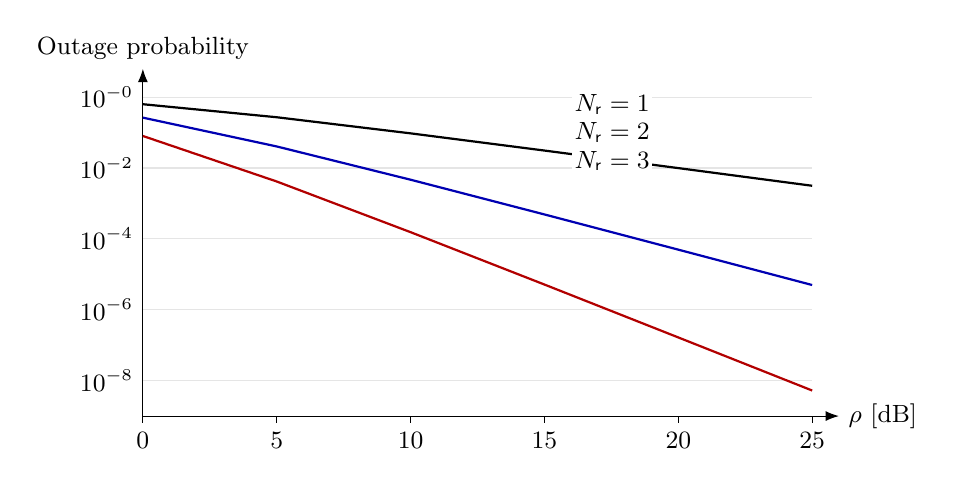
\begin{tikzpicture}[x=0.34cm,y=0.45cm,>=Latex,font=\small]
		\foreach \yy in {0,2,4,6,8} {
			\draw[gray!20] (0,-\yy)--(25,-\yy);
			\node[left] at (0,-\yy){$10^{-\yy}$};
		}
		\draw[->] (0,-9)--(26,-9) node[right]{$\rho$ [dB]};
		\draw[->] (0,-9)--(0,.8) node[above]{Outage probability};
		\foreach \xx in {0,5,10,15,20,25} {
			\draw (\xx,-9)--(\xx,-9.2);
			\node[below] at (\xx,-9.2){\xx};
		}
		\draw[thick,black] plot coordinates {
			(0,-0.19920) (5,-0.56686) (10,-1.02153)
			(15,-1.50685) (20,-2.00217) (25,-2.50069)
		};
		\draw[thick,blue!70!black] plot coordinates {
			(0,-0.57800) (5,-1.39136) (10,-2.32986)
			(15,-3.31017) (20,-4.30392) (25,-5.30195)
		};
		\draw[thick,red!70!black] plot coordinates {
			(0,-1.09528) (5,-2.38032) (10,-3.81064)
			(15,-5.28844) (20,-6.78141) (25,-8.27918)
		};
		\node[right,fill=white,inner sep=1pt] at (16,-0.2){$\NR=1$};
		\node[right,fill=white,inner sep=1pt] at (16,-1.0){$\NR=2$};
		\node[right,fill=white,inner sep=1pt] at (16,-1.8){$\NR=3$};
	\end{tikzpicture}
	\caption{Analytic Rayleigh MRC outage for $R_0=1$ bit/use and $\beta=1$. The logarithmic vertical axis illustrates diversity orders $\odiv=1,2,3$ for $\NR=1,2,3$.}
	\label{fig:outage}
\end{figure}


\subsection{Transmit diversity and the role of CSIT}

Consider a \ac{miso} channel with $\NT$ transmit ports and $\NR=1$. The channel vector $\ma{h}\in\compl^{\NT\times1}$ has independent entries $h_{\nT}\sim\CNormal(0,\beta)$, and the received signal is $y=\mT{\ma{h}}\ma{x}+v$.

\paragraph{Maximum-ratio transmission.}
With perfect instantaneous \ac{csit}, \ac{mrt} uses
\begin{equation*}
	\ma{f}_{\MRT}
	=\frac{\mC{\ma{h}}}{\NormTwo{\ma{h}}},
	\qquad
	\gamma_{\MRT}=\rho\NormTwo{\ma{h}}^2.
\end{equation*}
The output \ac{snr} has the same distribution as receive MRC with $\NT$ independent receive ports. Consequently, its fixed-rate outage diversity order is $\odiv=\NT$, under the same total transmit-energy constraint $\Ed$.

\paragraph{Fixed beamforming without instantaneous CSIT.}
For a fixed unit-norm beam $\ma{f}$, independent of the channel,
\begin{equation*}
	y=\mT{\ma{h}}\ma{f}\,d+v,
	\qquad
	\mT{\ma{h}}\ma{f}\sim\CNormal(0,\beta).
\end{equation*}
The effective scalar channel remains Rayleigh distributed, with diversity order $\odiv=1$, regardless of $\NT$.

Thus, multiple transmit ports do not automatically provide transmit diversity. Without instantaneous \ac{csit}, a suitable transmission scheme, such as space-time coding, is needed to exploit the independent fading coefficients.


\subsection{Transmit diversity through orthogonal space-time coding}

Orthogonal space-time block codes (\ac{ostbc}) distribute information symbols across transmit ports and channel uses. Their orthogonal structure permits simple coherent detection and can provide transmit diversity without instantaneous \ac{csit}.

\paragraph{Alamouti coding.}
For $\NT=2$, the Alamouti code from Lecture~02 transmits two information symbols over two channel uses:
\begin{equation*}
	\ma{X}
	=\frac{1}{\sqrt{2}}
	\begin{bmatrix}
		d_1&d_2\\
		-d_2^*&d_1^*
	\end{bmatrix}.
\end{equation*}
With $\NR$ receive ports, a channel constant over both channel uses, and perfect \ac{csir}, the information symbols can be detected separately without mutual interference.

For the normalization adopted in Lecture~02, the effective symbol \ac{snr} is
\begin{equation}\label{eq:alamouti-snr}
	\boxed{
		\gamma_{\mathsf A}
		=\frac{\rho}{2}\frob{\ma{H}}^2
		=\frac{\rho}{2}
		\sum_{\nR=1}^{\NR}\sum_{\nT=1}^{2}
		\Abs{h_{\nR\nT}}^2.
	}
\end{equation}
Under independent Rayleigh fading, the effective channel gain is the sum of $2\NR$ independent exponential random variables. For a fixed positive target rate, its outage probability therefore decreases asymptotically as $\rho^{-2\NR}$, giving
\begin{equation*}
	\boxed{\odiv=2\NR.}
\end{equation*}

The factor $1/2$ reflects the distribution of the total transmit energy over two transmit ports. The Alamouti code rate is one information symbol per channel use, so no additional time-rate reduction is introduced.

\paragraph{Comparison with beamforming.}
For $\NT=2$ and $\NR=1$, fixed beamforming without instantaneous \ac{csit} provides diversity order one. Alamouti coding without instantaneous \ac{csit} and MRT with perfect instantaneous \ac{csit} both achieve diversity order two.

The equal diversity orders do not imply equal outage probabilities. MRT optimizes the transmit direction for each realization, whereas Alamouti coding exploits independent channel gains through its space-time structure.

\paragraph{General OSTBC properties.}
For a normalized orthogonal code using $\NT$ transmit ports and $\NR$ receive ports, the effective symbol \ac{snr} can be expressed as
\begin{equation*}
	\gamma_{\mathsf{OSTBC}}
	=\frac{\rho}{\NT}\frob{\ma{H}}^2,
\end{equation*}
when the symbol and code-energy normalization is chosen consistently with the total average transmit energy per channel use $\Ed$.
%
Under independent Rayleigh fading, this gain contains $\NT\NR$ independent squared channel magnitudes, allowing full diversity order
\begin{equation*}
	\boxed{\odiv=\NT\NR.}
\end{equation*}

The code rate $R_{\mathsf c}$, in information symbols per channel use, must also be considered. The corresponding Gaussian-symbol rate benchmark has the form
\begin{equation*}
	R_{\mathsf{OSTBC}}(\ma{H})
	=R_{\mathsf c}\log_2(1+\gamma_{\mathsf{OSTBC}}).
\end{equation*}
Unlike the two-transmit Alamouti code, complex orthogonal designs with more than two transmit ports generally have $R_{\mathsf c}<1$.
%
Thus, full diversity does not necessarily imply maximum spectral efficiency or spatial multiplexing. Space-time coding and independent-stream transmission exploit the available spatial dimensions for different objectives.



\subsection{Effect of spatial correlation on diversity}

For correlated Rayleigh fading, consider the receive channel
\begin{equation*}
	\ma{h}=\sqrt{\beta}\ma{R}^{1/2}\ma{g},
	\qquad
	\ma{g}\sim\CNormal(\ma{0},\ma{I}_{\NR}),
\end{equation*}
where $\ma{R}\in\compl^{\NR\times\NR}$ is the spatial correlation matrix with rank $q\geq1$.
%
With MRC, the instantaneous \ac{snr} is
\begin{equation*}
	\gamma_{\MRC}
	=\rho\NormTwo{\ma{h}}^2
	=\rho\beta\mH{\ma{g}}\ma{R}\ma{g}.
\end{equation*}
Unlike independent Rayleigh fading, the combined \ac{snr} does not generally follow a Gamma distribution. Its distribution depends on the eigenvalues of $\ma{R}$, and the outage probability becomes
\begin{equation}\label{eq:corrout}
	P_{\mathsf{out},\MRC}(R_0)
	=\Prob{\NormTwo{\ma{h}}^2<a},
	\qquad
	a=\frac{2^{R_0}-1}{\rho}.
\end{equation}

Using the eigendecomposition
\begin{equation*}
	\ma{R}=\ma{Q}\diag{\lambda_1,\ldots,\lambda_q,0,\ldots,0}\mH{\ma{Q}},
\end{equation*}
where $\ma{Q}$ is unitary and $\lambda_1,\ldots,\lambda_q>0$, and defining $\ma{u}=\mH{\ma{Q}}\ma{g}$, the channel gain becomes
\begin{equation}\label{eq:corrgain}
	\boxed{
		\NormTwo{\ma{h}}^2
		=\beta\sum_{i=1}^{q}\lambda_i\Abs{u_i}^2.
	}
\end{equation}
The vector $\ma{u}\in\compl^{\NR\times1}$ has independent $\CNormal(0,1)$ entries due to the unitary transformation. Therefore, the channel gain is a weighted sum of independent exponential random variables. For equal positive eigenvalues, its distribution reduces to a scaled Gamma distribution.

For small positive $a$, the cumulative distribution function satisfies
\begin{equation}\label{eq:corrtail}
	\boxed{
		\lim_{a\to0^+}
		\frac{\Prob{\NormTwo{\ma{h}}^2<a}}{a^q}
		=
		\frac{1}{q!\,\beta^q\prod_{i=1}^{q}\lambda_i}.
	}
\end{equation}
Thus, the outage probability decreases proportionally to $a^q$. Since $a\propto1/\rho$, the asymptotic diversity order is
\begin{equation*}
	\boxed{\odiv=q=\rank{\ma{R}}.}
\end{equation*}
Full-rank correlation preserves the maximum diversity order $\NR$, although strong correlation can degrade outage performance at practical \ac{snr}. Only exact rank deficiency reduces the asymptotic diversity order.

\begin{example}{Fully correlated receive ports}
	Consider $\ma{h}=g\ma{1}_{\NR}$, where $g\sim\CNormal(0,\beta)$. MRC gives
	\begin{equation*}
		\gamma_{\MRC}
		=\NR\rho\Abs{g}^2.
	\end{equation*}
	The mean output \ac{snr} increases by $\NR$, but all receive ports experience the same fading coefficient. The correlation matrix has rank one, giving diversity order $\odiv=1$.
	
	Thus, array gain can remain even when independent fading observations are lost.
\end{example}


\subsection{Diversity--multiplexing tradeoff: conceptual view}

Diversity improves reliability, whereas spatial multiplexing increases the achievable rate. At high \ac{snr}, their interaction can be characterized by the diversity--multiplexing tradeoff (\ac{dmt}).

For a family of communication schemes, the multiplexing gain is defined as
\begin{equation}\label{eq:multiplexinggain}
	\boxed{
		\gmux
		=\lim_{\rho\to\infty}
		\frac{R(\rho)}{\log_2\rho}.
	}
\end{equation}
Thus, $\gmux$ describes how the transmission rate increases with \ac{snr}, rather than the number of simultaneously transmitted streams.

\paragraph{Diversity order: outage and error probability.}
The diversity order introduced in Section~\ref{sec:diversity} describes the asymptotic decay of outage probability at a fixed target rate. More generally, for an \ac{snr}-dependent rate $R(\rho)$, the outage diversity order is
\begin{equation*}
	\odiv^{\mathsf{out}}(\gmux)
	=-\lim_{\rho\to\infty}
	\frac{\ln P_{\mathsf{out}}(R(\rho);\rho)}
	{\ln\rho}.
\end{equation*}
An equivalent scaling measure can be defined using the codeword error probability:
\begin{equation}\label{eq:dmtdiversity}
	\boxed{
		\odiv^{\mathsf{err}}(\gmux)
		=-\lim_{\rho\to\infty}
		\frac{\ln P_{\mathsf e}(\rho)}
		{\ln\rho}.
	}
\end{equation}
For quasi-static fading, outage provides a fundamental reliability benchmark. With suitable coding and decoding, the optimal error-probability diversity order can attain the outage diversity order:
\begin{equation*}
	\boxed{
		\odiv(\gmux)
		=\odiv^{\mathsf{out}}(\gmux)
		=\odiv^{\mathsf{err}}(\gmux).
	}
\end{equation*}
This equality concerns optimal asymptotic performance under the stated assumptions. Particular codes and receivers may achieve a smaller error-probability diversity order.

\paragraph{Optimal DMT of independent Rayleigh MIMO.}
For quasi-static \ac{iid} Rayleigh \ac{mimo}, perfect \ac{csir}, no instantaneous \ac{csit}, a short-term transmit-energy constraint, and sufficiently long suitable space-time codes, the optimal tradeoff is a piecewise-linear function $\odiv(\gmux)$. The curve connects the points
\begin{equation}\label{eq:dmt}
	\boxed{
		\gmux=\ell,\qquad
		\odiv(\ell)=(\NT-\ell)(\NR-\ell),
		\quad
		\ell=0,1,\ldots,\min(\NT,\NR).
	}
\end{equation}
Between consecutive integer values of $\gmux$, the diversity order is obtained by linear interpolation.

For example, a $2\times2$ channel gives
\begin{equation*}
	\odiv(0)=4,\qquad
	\odiv(1)=1,\qquad
	\odiv(2)=0,
\end{equation*}
and therefore
\begin{equation*}
	\odiv(\gmux)=
	\begin{cases}
		4-3\gmux,
		&0\leq\gmux\leq1,\\
		2-\gmux,
		&1\leq\gmux\leq2.
	\end{cases}
\end{equation*}
%
At a fixed positive transmission rate, $\gmux=0$, and diversity order four is achievable using suitable coding. At the maximum rate scaling $\gmux=2$, the diversity exponent becomes zero.
%
Thus, increasing the transmission rate with \ac{snr} reduces the asymptotic improvement in reliability. The DMT provides an optimal coding benchmark, not a performance guarantee for uncoded spatial multiplexing or a particular linear equalizer.


\section{Summary and transition to multiuser MIMO}

Lecture~02 introduced signal processing and achievable rates for a given MIMO channel. This lecture extended the analysis to random channels, where channel realizations and their associated performance vary according to statistical distributions.

\begin{itemize}
	\item \textbf{Statistical channel models:} Rayleigh, Rician, and correlated fading models describe scattering, deterministic propagation components, and spatial dependence. Consistent channel normalization is essential.
	
	\item \textbf{Spatial channel properties:} Antenna counts and channel statistics determine the available spatial dimensions. Exact rank, conditioning, effective rank, and active stream count characterize different aspects of spatial multiplexing.
	
	\item \textbf{Performance metrics:} Ergodic rate describes average achievable rate, while outage probability measures the risk that a channel realization cannot support a target rate. Their operational interpretation depends on the coding horizon and transmission scheme.
	
	\item \textbf{Diversity and array gain:} Diversity order characterizes the high-\ac{snr} decay of error or outage probability, whereas array gain describes improvements in received signal strength. Both depend on the transmission and reception scheme.
	
	\item \textbf{Transmit diversity and multiplexing:} Channel adaptation and space-time coding can exploit multiple transmit ports for diversity. Increasing multiplexing gain can reduce the asymptotic reliability improvement, as illustrated by the diversity--multiplexing tradeoff.
\end{itemize}

\paragraph{Transition to multiuser MIMO.}
The next lectures extend the point-to-point system to multiple users. Unlike a single cooperating receiver, users may occupy different locations and decode their signals independently. Spatial processing must therefore account for interuser interference, user-specific channels, and resource allocation. The channel statistics, spatial properties, and performance metrics introduced in this lecture provide the foundation for analyzing these systems.

\section*{Further reading}
\begin{itemize}
	\item D.~Tse and P.~Viswanath, \emph{Fundamentals of Wireless Communication}, Cambridge University Press, 2005, Chapters~3, 7--9.
	\item A.~Paulraj, R.~Nabar, and D.~Gore, \emph{Introduction to Space-Time Wireless Communications}, Cambridge University Press, 2003.
	\item A.~Goldsmith, \emph{Wireless Communications}, Cambridge University Press, 2005.
	\item L.~Zheng and D.~N.~C. Tse, ``Diversity and Multiplexing: A Fundamental Tradeoff in Multiple-Antenna Channels,'' \emph{IEEE Transactions on Information Theory}, vol.~49, no.~5, pp.~1073--1096, 2003.
\end{itemize}

\clearpage

\section*{Review questions: channel statistics and performance}

Unless otherwise stated, assume $\beta=1$, white Gaussian noise, total transmit-energy budget $\Ed$, and perfect \ac{csir}. Rates are measured in bit per complex channel use. State any additional \ac{csit} assumptions where relevant.

\begin{enumerate}[label=\textbf{E\arabic*.}]
	
	\item Let $g=(a+jb)/\sqrt{2}$, where $a,b\sim\Normal(0,1)$ are independent. Find $\Ex{g}$, $\Ex{\Abs{g}^2}$, and $\Var{\RE{g}}$. What changes if the factor $1/\sqrt{2}$ is omitted?
	
	\item A $3\times2$ independent Rayleigh channel has coefficient variance $\beta=0.2$. Find its expected squared Frobenius norm. Does the channel have rank two for every realization or almost surely?
	
	\item Consider the spatial correlation matrix $\ma{R}(0.9)$ from \eqref{eq:correlation}. Find its eigenvalues, trace, and rank. If both Kronecker correlation factors equal $\ma{R}(0.9)$, determine the expected squared channel norm and the almost-sure channel rank for $\beta=1$.
	
	\item Consider a $2\times2$ Rician channel with $\kappa=9$, $\beta=1$, and $\frob{\ma{H}_{\mathsf{det}}}^2=4$. Determine the deterministic power, average scattered power, and total average channel power.
	
	\item A $2\times2$ channel has squared singular values $(1,0.01)$. Find its exact rank, condition number $\mathsf{cond}_{H}$, and effective rank. For $\sigma_v^2=1$, determine the minimum transmit energy required to activate the second mode through water-filling.
	
	\item For SISO Rayleigh fading at $\rho=10$, calculate the outage probability at $R_0=1$ bit/use and the $10\%$ outage rate. Compare the latter with the ergodic rate of approximately $2.907$ bit/use.
	
	\item For the same $\rho$, $\beta$, and $R_0$, calculate the outage probability of independent two-port receive MRC. Why is $(1-e^{-0.1})^2$ not the correct MRC outage probability? Which combining scheme does it describe?
	
	\item Compare independent two-port receive MRC with the fully correlated channel $\ma{h}=g[1,1]^{\mathsf T}$, where $g\sim\CNormal(0,1)$. Determine the mean output \ac{snr} and diversity order for both cases.
	
	\item Consider two transmit ports with independent Rayleigh fading and one receive port. Compare fixed unit-norm beamforming, MRT, and Alamouti coding in terms of instantaneous \ac{csit}, effective symbol \ac{snr}, and diversity order. Assume perfect \ac{csir} and the same total transmit-energy budget.
	
	\item For the optimal $2\times2$ diversity--multiplexing tradeoff, determine $\odiv(0.5)$ and $\odiv(1.5)$, where the argument denotes $\gmux$. Does channel rank $\RH=2$ imply that diversity order and multiplexing gain are both two?
	
	\item Does increasing the Rician factor $\kappa$ necessarily improve ergodic rate or reduce outage probability? Explain how the deterministic channel structure and the selected transmission scheme affect the answer.
	
\end{enumerate}


\clearpage
\subsection*{Answers}

\begin{enumerate}[label=\textbf{E\arabic*.}]
	
	\item $\Ex{g}=0$, $\Ex{\Abs{g}^2}=1$, and $\Var{\RE{g}}=1/2$. Without the normalization, the average coefficient power becomes $2$, corresponding to a $3.01$ dB increase.
	
	\item $\Ex{\frob{\ma{H}}^2}=3\cdot2\cdot0.2=1.2$. The rank is two almost surely; exact linear dependence occurs with probability zero.
	
	\item The eigenvalues are $1.9$ and $0.1$, giving trace $2$ and rank $2$. The Kronecker channel has $\Ex{\frob{\ma{H}}^2}=2\cdot2=4$ and rank two almost surely.
	
	\item The deterministic power is $4\cdot9/10=3.6$, the average scattered power is $4/10=0.4$, and the total average power is $4$. The Rician model scales amplitudes by the square roots of the corresponding power fractions.
	
	\item The exact rank is $2$, $\mathsf{cond}_{H}=10$, and the effective rank is approximately $1.057$. The second mode receives positive energy only when $\Ed>99$; at $\Ed=99$, its allocation is zero.
	
	\item The outage probability is $1-e^{-0.1}\approx0.09516$. The $10\%$ outage rate is $\log_2(1-10\ln0.9)\approx1.038$ bit/use. The ergodic rate describes average performance, whereas the outage rate characterizes a lower quantile of the supported-rate distribution.
	
	\item The MRC outage probability is $1-e^{-0.1}(1+0.1)\approx0.004679$. The expression $(1-e^{-0.1})^2\approx0.009056$ describes selection combining: both individual channel gains are below the threshold. MRC instead fails when their sum is below the threshold.
	
	\item Both channels have mean output \ac{snr} $2\rho$. Independent fading gives $\odiv=2$, while complete correlation gives $\odiv=1$. Both obtain array gain, but only the independent channel provides second-order diversity.
	
	\item Fixed beamforming requires no instantaneous \ac{csit} and gives $\gamma=\rho\Abs{g}^2$, where $g\sim\CNormal(0,1)$, with diversity order one. MRT requires instantaneous \ac{csit} and gives $\gamma=\rho(\Abs{h_1}^2+\Abs{h_2}^2)$, with diversity order two. Alamouti coding requires no instantaneous \ac{csit} and gives $\gamma=(\rho/2)(\Abs{h_1}^2+\Abs{h_2}^2)$, also with diversity order two. All three assume perfect \ac{csir}.
	
	\item $\odiv(0.5)=2.5$ and $\odiv(1.5)=0.5$. The exact channel rank describes available spatial dimensions, whereas the DMT characterizes the asymptotic tradeoff between rate scaling and reliability for suitable code families.
	
	\item No universal improvement is guaranteed. Increasing $\kappa$ changes the balance between deterministic and scattered components. The effect on ergodic rate and outage depends on the singular-value structure of $\ma{H}_{\mathsf{det}}$, the transmission covariance, the target rate, and the available \ac{csit}. A stronger deterministic component can improve reliability for some schemes and rate targets while reducing useful spatial multiplexing opportunities for others.
\end{enumerate}

% ============================================================
% Mathematical appendices — Lecture 03
% ============================================================
\clearpage
\appendix

\section{Jensen's inequality and average achievable rate}
\label{app:jensen}


\subsection{Jensen's inequality}

A function $f(x)$ is concave if, for any $x_1,x_2$ and $0\leq\theta\leq1$,
\begin{equation*}
	f(\theta x_1+(1-\theta)x_2)
	\geq\theta f(x_1)+(1-\theta)f(x_2).
\end{equation*}
This property extends to weighted sums:
\begin{equation*}
	f\left(\sum_{n=1}^{N}p_nx_n\right)
	\geq\sum_{n=1}^{N}p_nf(x_n),
	\qquad
	\sum_{n=1}^{N}p_n=1,\quad p_n\geq0.
\end{equation*}
Similarly, for a nonnegative weighting function $g(x)$ satisfying $\int_{\mathcal X}g(x)\,dx=1$,
\begin{equation*}
	f\left(\int_{\mathcal X}xg(x)\,dx\right)
	\geq\int_{\mathcal X}f(x)g(x)\,dx.
\end{equation*}

For a random variable $X$ with \ac{pdf} $f_X(x)$, choosing $g(x)=f_X(x)$ gives Jensen's inequality:
\begin{equation}\label{eq:app-jensen}
	\boxed{
		\Ex{f(X)}\leq f(\Ex{X}),
	}
\end{equation}
provided $f$ is concave on the support of $X$ and the expectations exist.

\paragraph{Proof using the tangent line.}
For a differentiable concave function, the tangent line at any point $m$ lies above its graph:
\begin{equation*}
	f(x)\leq f(m)+f'(m)(x-m).
\end{equation*}
Setting $m=\Ex{X}$ and taking expectations gives
\begin{align*}
	\Ex{f(X)}
	&\leq f(m)+f'(m)\Ex{X-m}\\
	&=f(m)=f(\Ex{X}).
\end{align*}
For a strictly concave function, equality holds only if $X$ is constant almost surely, assuming the expectations are well defined.


\subsection{Application to the ergodic rate}
The function $f(x)=\log_2(1+x)$ is strictly concave for $x\geq0$, since
\begin{equation*}
	f''(x)=-\frac{1}{(1+x)^2\ln 2}<0.
\end{equation*}
Applying Jensen's inequality to the instantaneous received \ac{snr} $\gamma$ gives
\begin{equation}\label{eq:app-jensen-snr}
	\overline R
	=\Ex{\log_2(1+\gamma)}
	\leq\log_2(1+\Ex{\gamma}).
\end{equation}
For scalar Rayleigh fading with $h=\sqrt{\beta}\,g$, $g\sim\CNormal(0,1)$, and $\gamma=\rho\beta\Abs{g}^2$, the unit average power $\Ex{\Abs{g}^2}=1$ yields
\begin{equation}\label{eq:app-jensen-rayleigh}
	\boxed{
		\overline R_{\mathsf{SISO}}
		\leq\log_2(1+\rho\beta).
	}
\end{equation}
The inequality is strict for $\rho\beta>0$.


\subsection{Extension to MIMO}

For a fixed transmit covariance $\ma{R}_x$, the instantaneous Gaussian achievable rate is
\begin{equation*}
	R(\ma{H})
	=\log_2\Det{
		\ma{I}_{\NR}
		+\sigma_v^{-2}\ma{H}\ma{R}_x\mH{\ma{H}}
	}.
\end{equation*}
The function
$\log_2\Det{\ma{I}+\ma{X}}$
is concave over Hermitian positive-semidefinite matrices $\ma{X}$. 
Applying the matrix form of Jensen's inequality gives
\begin{equation}\label{eq:app-jensen-mimo}
	\overline R
	=\Ex{\log_2\Det{
			\ma{I}_{\NR}
			+\sigma_v^{-2}\ma{H}\ma{R}_x\mH{\ma{H}}
	}}
	\leq
	\log_2\Det{
		\ma{I}_{\NR}
		+\sigma_v^{-2}
		\Ex{\ma{H}\ma{R}_x\mH{\ma{H}}}
	}.
\end{equation}
The transmit covariance is assumed fixed and
independent of the channel realization.


For independent Rayleigh fading with
$\Ex{\Abs{h_{\nR\nT}}^2}=\beta$, the expected matrix product satisfies
\begin{equation*}
	\Ex{\ma{H}\ma{R}_x\mH{\ma{H}}}
	=\beta\trace{\ma{R}_x}\ma{I}_{\NR}.
\end{equation*}
For isotropic transmission with
$\trace{\ma{R}_x}=\Ed$,
\begin{equation*}
	\overline R_{\mathsf{iso}}
	\leq\NR\log_2(1+\rho\beta).
\end{equation*}
This is an upper bound, not an exact expression for the ergodic MIMO rate.


% ============================================================

\section{Rayleigh power distributions and MRC outage}
\label{app:rayleigh-gamma}


\subsection{Transformation of random variables}

\paragraph{Change of variables in a probability density.}
Consider a continuous random variable $X$ with \ac{pdf} $f_X(x)$ and a transformation $Y=T(X)$. If $T$ is differentiable and one-to-one, the probability is preserved under the transformation:
\begin{equation*}
	f_Y(y)\,dy=f_X(x)\,|dx|.
\end{equation*}
Consequently, the transformed density is
\begin{equation}\label{eq:app-pdf-transform}
	\boxed{
		f_Y(y)=f_X(T^{-1}(y))
		\left|\frac{dT^{-1}(y)}{dy}\right|.
	}
\end{equation}
The absolute value accounts for transformations with negative derivatives. For transformations with multiple inverse solutions $x_i$, the contributions from all solutions must be summed.

For a transformation of two random variables $(X_1,X_2)$ into $(Y_1,Y_2)$, the corresponding result uses the Jacobian determinant:
\begin{equation}\label{eq:app-pdf-jacobian}
	f_{Y_1,Y_2}(y_1,y_2)
	=f_{X_1,X_2}(x_1,x_2)
	\left|
	\det{\frac{\partial(x_1,x_2)}
		{\partial(y_1,y_2)}}
	\right|.
\end{equation}
Here $(x_1,x_2)$ denotes the inverse transformation evaluated at $(y_1,y_2)$.

\paragraph{Rayleigh amplitude distribution.}
Consider the normalized complex Gaussian variable
\begin{equation*}
	g=\frac{a+jb}{\sqrt{2}},
	\qquad
	a,b\sim\Normal(0,1),
\end{equation*}
where $a$ and $b$ are independent. Its real and imaginary parts have variance $1/2$, giving the joint density
\begin{equation*}
	f_{\RE{g},\IM{g}}(x,y)
	=\frac{1}{\pi}e^{-(x^2+y^2)}.
\end{equation*}

Using polar coordinates
\begin{equation*}
	x=r\cos\varphi,\qquad
	y=r\sin\varphi,
\end{equation*}
the Jacobian determinant of the inverse transformation is
\begin{equation*}
	\left|
	\det{
		\begin{bmatrix}
			\cos\varphi&-r\sin\varphi\\
			\sin\varphi&r\cos\varphi
	\end{bmatrix}}
	\right|=r.
\end{equation*}
The joint density of amplitude and phase therefore becomes
\begin{equation*}
	f_{r,\varphi}(r,\varphi)
	=\frac{r}{\pi}e^{-r^2},
	\qquad
	r\geq0,\quad 0\leq\varphi<2\pi.
\end{equation*}
Integrating over the phase gives the Rayleigh amplitude density:
\begin{equation}\label{eq:app-rayleigh-pdf}
	\boxed{
		f_r(r)=\int_0^{2\pi}
		f_{r,\varphi}(r,\varphi)\,d\varphi
		=2re^{-r^2},\qquad r\geq0.
	}
\end{equation}

\paragraph{Exponential squared-amplitude distribution.}
Let $z=r^2=\Abs{g}^2$. The inverse transformation is $r=\sqrt{z}$, with
\begin{equation*}
	\frac{dr}{dz}=\frac{1}{2\sqrt{z}}.
\end{equation*}
Applying \eqref{eq:app-pdf-transform} gives
\begin{align*}
	f_z(z)
	&=f_r(\sqrt{z})
	\left|\frac{dr}{dz}\right|\\
	&=2\sqrt{z}e^{-z}
	\frac{1}{2\sqrt{z}}\\
	&=e^{-z},\qquad z\geq0.
\end{align*}
Integrating the density from $0$ to $z$ gives its cumulative distribution function:
\begin{equation*}
	F_z(z)=\int_0^z e^{-t}\,dt=1-e^{-z}.
\end{equation*}
Thus, the normalized squared amplitude follows an exponential distribution with unit mean:
\begin{equation}\label{eq:app-exponential}
	\boxed{
		f_z(z)=e^{-z},\qquad
		F_z(z)=1-e^{-z},\quad z\geq0.
	}
\end{equation}


\subsection{Laplace transforms and sums of random variables}

\paragraph{Laplace transform of a probability density.}
For a nonnegative random variable $X$ with \ac{pdf} $f_X(x)$, its Laplace transform is defined as
\begin{equation}\label{eq:app-laplace}
	\boxed{
		\mathcal{L}_X(t)
		=\Ex{e^{-tX}}
		=\int_0^\infty e^{-tx}f_X(x)\,dx,
		\qquad t\geq0.
	}
\end{equation}
The transform provides an alternative representation of the probability distribution. In particular, it simplifies the analysis of sums of independent random variables.

For independent nonnegative random variables $X_1,\ldots,X_N$, let
\begin{equation*}
	Z=\sum_{n=1}^{N}X_n.
\end{equation*}
Using the independence of the variables,
\begin{align*}
	\mathcal{L}_Z(t)
	&=\Ex{e^{-t\sum_{n=1}^{N}X_n}}\\
	&=\Ex{\prod_{n=1}^{N}e^{-tX_n}}\\
	&=\prod_{n=1}^{N}\Ex{e^{-tX_n}}.
\end{align*}
Therefore,
\begin{equation}\label{eq:app-laplace-sum}
	\boxed{
		\mathcal{L}_Z(t)
		=\prod_{n=1}^{N}\mathcal{L}_{X_n}(t).
	}
\end{equation}
Thus, the distribution of a sum, which would otherwise require convolution of the individual densities, can be determined through multiplication of their Laplace transforms.

\paragraph{Application to independent Rayleigh fading.}
For independent Rayleigh fading at $\NR$ receive ports, define
\begin{equation*}
	Z=\sum_{n_{\mathsf r}=1}^{\NR}
	\Abs{g_{n_{\mathsf r}}}^2,
	\qquad
	g_{n_{\mathsf r}}\sim\CNormal(0,1).
\end{equation*}
As shown in the previous subsection, each squared magnitude follows an exponential distribution with density $f_z(z)=e^{-z}$ for $z\geq0$.

Its Laplace transform is
\begin{align*}
	\mathcal{L}_{|g|^2}(t)
	&=\int_0^\infty e^{-tz}e^{-z}\,dz\\
	&=\int_0^\infty e^{-(1+t)z}\,dz\\
	&=\frac{1}{1+t}.
\end{align*}
Since all $\NR$ variables are independent, their sum has Laplace transform
\begin{equation}\label{eq:app-gamma-laplace}
	\boxed{
		\mathcal{L}_Z(t)
		=\left(\frac{1}{1+t}\right)^{\NR}.
	}
\end{equation}

\paragraph{Gamma distribution.}
The Gamma distribution with integer shape $\NR$ and unit scale has the density
\begin{equation*}
	f_Z(z)=\frac{z^{\NR-1}e^{-z}}{(\NR-1)!},
	\qquad z\geq0.
\end{equation*}
Its Laplace transform is
\begin{align*}
	\mathcal{L}_Z(t)
	&=\frac{1}{(\NR-1)!}
	\int_0^\infty z^{\NR-1}e^{-(1+t)z}\,dz\\
	&=\frac{1}{(1+t)^{\NR}},
\end{align*}
where the last step follows from the substitution $u=(1+t)z$ and the identity
\begin{equation*}
	\int_0^\infty u^{\NR-1}e^{-u}\,du
	=(\NR-1)!.
\end{equation*}
Comparing this transform with \eqref{eq:app-gamma-laplace} shows that the sum of $\NR$ independent unit-mean exponential variables follows a Gamma distribution with shape $\NR$ and unit scale:
\begin{equation}\label{eq:app-gamma-pdf}
	\boxed{
		f_Z(z)
		=\frac{z^{\NR-1}e^{-z}}{(\NR-1)!},
		\qquad z\geq0.
	}
\end{equation}
\subsection{Gamma CDF and MRC outage}

The cumulative distribution function is
\begin{equation*}
	F_Z(a)
	=\frac{1}{(\NR-1)!}
	\int_0^a z^{\NR-1}e^{-z}\,dz.
\end{equation*}
For integer $\NR$, the integral can be evaluated by repeated integration by parts.

Define
\begin{equation*}
	I_n(a)=\int_0^a z^ne^{-z}\,dz.
\end{equation*}
Integration by parts gives
\begin{equation*}
	I_n(a)
	=-a^ne^{-a}+nI_{n-1}(a),
\end{equation*}
with
\begin{equation*}
	I_0(a)=1-e^{-a}.
\end{equation*}
Repeated application yields
\begin{equation*}
	I_n(a)
	=n!\left(
	1-e^{-a}\sum_{\ell=0}^{n}
	\frac{a^\ell}{\ell!}
	\right).
\end{equation*}
Setting $n=\NR-1$ gives
\begin{equation}\label{eq:app-gamma-cdf}
	\boxed{
		F_Z(a)
		=1-e^{-a}
		\sum_{\ell=0}^{\NR-1}\frac{a^\ell}{\ell!}.
	}
\end{equation}

For MRC under independent Rayleigh fading,
\begin{equation*}
	\gamma_{\MRC}
	=\rho\beta Z.
\end{equation*}
At target rate $R_0$, outage occurs when
\begin{equation*}
	\log_2(1+\gamma_{\MRC})<R_0.
\end{equation*}
Equivalently,
\begin{equation*}
	Z<a,\qquad
	a=\frac{2^{R_0}-1}{\rho\beta}.
\end{equation*}
Substituting this threshold into the Gamma CDF gives
\begin{equation}\label{eq:app-mrc-outage}
	\boxed{
		P_{\mathsf{out},\MRC}(R_0)
		=1-e^{-a}
		\sum_{\ell=0}^{\NR-1}\frac{a^\ell}{\ell!}.
	}
\end{equation}

\subsection{High-SNR approximation and diversity order}

For fixed $R_0>0$ and $\beta>0$, the threshold $a$ approaches zero as $\rho\to\infty$. Expanding the Gamma CDF near zero, or using $e^{-z}\approx1$ inside its defining integral, gives
\begin{align*}
	F_Z(a)
	&=\frac{1}{(\NR-1)!}
	\int_0^a z^{\NR-1}e^{-z}\,dz\\
	&\approx
	\frac{1}{(\NR-1)!}
	\int_0^a z^{\NR-1}\,dz\\
	&=\frac{a^{\NR}}{\NR!}.
\end{align*}
Therefore,
\begin{equation*}
	P_{\mathsf{out},\MRC}(R_0)
	\approx
	\frac{(2^{R_0}-1)^{\NR}}
	{\NR!(\rho\beta)^{\NR}},
	\qquad \rho\to\infty.
\end{equation*}
The outage probability decreases proportionally to $\rho^{-\NR}$. Hence,
\begin{equation*}
	\boxed{\odiv=\NR.}
\end{equation*}
The same derivation applies to independent Rayleigh MRT with $\NT$ transmit ports, replacing $\NR$ by $\NT$, when perfect instantaneous \ac{csit} is available.



\section{Diversity order under spatially correlated fading}
\label{app:correlated-diversity}

\subsection{Distribution of the combined channel gain}

As derived in Section~\ref{sec:diversity}, the squared norm of a correlated Rayleigh channel can be expressed as
\begin{equation*}
	G=\NormTwo{\ma{h}}^2
	=\beta\sum_{i=1}^{q}\lambda_i\Abs{u_i}^2,
\end{equation*}
where $q=\rank{\ma{R}}$, $\lambda_i>0$ are its positive eigenvalues, and $u_i$ are independent $\CNormal(0,1)$ variables.
%
Using the Laplace-transform properties introduced in Appendix~\ref{app:rayleigh-gamma}, the transform of $G$ is
\begin{equation}\label{eq:app-corr-laplace}
	\mathcal{L}_G(t)
	=\prod_{i=1}^{q}\frac{1}{1+t\beta\lambda_i}.
\end{equation}


For large $t$, the Laplace transform is dominated
by the density near $x=0$, due to the weighting
factor $e^{-tx}$. In particular,
\begin{equation*}
	\mathcal{L}_G(t)
	\approx
	\frac{1}{
		t^q\beta^q\prod_{i=1}^{q}\lambda_i
	},
	\qquad t\to\infty.
\end{equation*}
Using the inverse Laplace relation
\begin{equation*}
	\mathcal{L}^{-1}\{t^{-q}\}
	=\frac{x^{q-1}}{(q-1)!},
\end{equation*}
the leading small-$x$ behavior is
\begin{equation*}
	f_G(x)\approx
	\frac{x^{q-1}}{
		(q-1)!\,\beta^q
		\prod_{i=1}^{q}\lambda_i
	},
	\qquad x\to0^+.
\end{equation*}


Integrating from zero to $a$ gives
\begin{equation}\label{eq:app-corr-tail}
	\boxed{
		\lim_{a\to0^+}
		\frac{\Prob{G<a}}{a^q}
		=
		\frac{1}{q!\,\beta^q\prod_{i=1}^{q}\lambda_i}.
	}
\end{equation}

\subsection{Outage diversity order}

For MRC, $\gamma_{\MRC}=\rho G$. At a fixed target rate $R_0>0$, outage occurs when
\begin{equation*}
	G<a,\qquad
	a=\frac{2^{R_0}-1}{\rho}.
\end{equation*}
Applying \eqref{eq:app-corr-tail}, the high-\ac{snr} outage probability becomes
\begin{equation*}
	P_{\mathsf{out},\MRC}(R_0)
	\approx
	\frac{(2^{R_0}-1)^q}
	{q!\,\beta^q\prod_{i=1}^{q}\lambda_i}
	\rho^{-q}.
\end{equation*}
Consequently,
\begin{equation*}
	\odiv
	=-\lim_{\rho\to\infty}
	\frac{\ln P_{\mathsf{out},\MRC}(R_0)}
	{\ln\rho}
	=q=\rank{\ma{R}}.
\end{equation*}


\section{Outage and error-probability diversity}
\label{app:outage-error}

The diversity order describes the asymptotic decay of a reliability metric with increasing \ac{snr}. It can be defined using outage probability, codeword error probability, or bit-error probability:
\begin{align*}
	\odiv^{\mathsf{out}}
	&=-\lim_{\rho\to\infty}
	\frac{\ln P_{\mathsf{out}}(R_0;\rho)}{\ln\rho},\\
	\odiv^{\mathsf{err}}
	&=-\lim_{\rho\to\infty}
	\frac{\ln P_{\mathsf e}(\rho)}{\ln\rho},\\
	\odiv^{\mathsf{bit}}
	&=-\lim_{\rho\to\infty}
	\frac{\ln \overline P_{\mathsf b}(\rho)}{\ln\rho}.
\end{align*}
Outage characterizes the probability that a channel realization cannot support a target rate, independently of a particular code. In contrast, codeword and bit-error probabilities depend on the modulation, coding, and receiver. Their diversity orders may coincide, although the corresponding probabilities and their interpretations differ.
%
For quasi-static fading, outage provides an information-theoretic reliability benchmark. Under suitable coding and decoding assumptions, the optimal codeword-error diversity order can attain the outage diversity order. This equality is not guaranteed for arbitrary transmission schemes.

\begin{example}{SISO Rayleigh fading: outage versus BPSK error}
	
	For scalar Rayleigh fading with a fixed target rate $R_0>0$, the outage probability is
	\begin{equation*}
		P_{\mathsf{out}}(R_0)
		=1-\exp\left(
		-\frac{2^{R_0}-1}{\rho\beta}
		\right).
	\end{equation*}
	Using $1-e^{-x}\approx x$ for small $x$ gives
	\begin{equation*}
		P_{\mathsf{out}}(R_0)
		\approx\frac{2^{R_0}-1}{\rho\beta},
		\qquad \rho\to\infty.
	\end{equation*}
	Therefore, $\odiv^{\mathsf{out}}=1$.
	
	For coherent uncoded \ac{bpsk}, the average bit-error probability is
	\begin{equation*}
		\overline P_{\mathsf b}
		=\frac12\left(
		1-\sqrt{\frac{\rho\beta}{1+\rho\beta}}
		\right).
	\end{equation*}
	Using $(1+x)^{-1/2}\approx1-x/2$ for small $x$,
	\begin{align*}
		\overline P_{\mathsf b}
		&=\frac12\left[
		1-\left(1+\frac{1}{\rho\beta}\right)^{-1/2}
		\right]\\
		&\approx\frac{1}{4\rho\beta},
		\qquad \rho\to\infty.
	\end{align*}
	Consequently, $\odiv^{\mathsf{bit}}=1$.
	
	Both outage probability and uncoded BPSK bit-error probability decrease proportionally to $\rho^{-1}$ and therefore exhibit the same diversity order, despite their different coefficients and interpretations. This example illustrates matching asymptotic exponents, not a general equivalence between outage, bit-error, and codeword error probabilities.
\end{example}


\end{document}
